\documentclass{article}

\title{Interactively Reviewing State of the Art Prime Editing Guide RNA Design Models}
\author{Peiheng Lu}
% line number
\usepackage{lineno}
\linenumbers

\usepackage{graphicx}
\usepackage{amsmath}
\usepackage[sorting=none]{biblatex}
\usepackage{hyperref}
\usepackage{xurl}
\urlstyle{tt}

\addbibresource{term-paper.bib}
\graphicspath{diagrams/illustration/}


% increase text width
\usepackage{geometry}
\geometry{a4paper, margin=1in}
\usepackage{longtable}
\usepackage{array}

% Word count via texcount (requires compiling with -shell-escape)
\makeatletter
\newcommand{\wordcountwords}{%
  \immediate\write18{texcount -inc -sum -1 -q \jobname.tex > \jobname.wc}%
  \IfFileExists{\jobname.wc}{\input{\jobname.wc}\unskip}{---}%
}
\makeatother
\date{\today\qquad Word count: \wordcountwords}


\begin{document}

\maketitle

\begin{abstract}

Prime editing can install substitutions, insertions, and deletions without double-strand DNA breaks, but its efficiency depends strongly on pegRNA sequence, edit type, and experimental context. Although several predictive models have been published, differences in datasets, input representations, checkpoints, and evaluation protocols make their performance difficult to compare. Here, I present PE Hub, a unified platform for curating prime-editing data and benchmarking, training, and combining pegRNA efficiency models. PE Hub comprises a database that standardizes approximately 756,000 pegRNA--target pairs from seven studies, a model service integrating DeepPrime, OPED, PRIDICT2, and OptiPrime, and a web interface and command-line workflow for reproducible experiments. Model-specific input conversion, locus-grouped partitioning, checkpoint provenance, and protospacer-level leakage checks enable comparisons across heterogeneous datasets while retaining each model's native representation. Evaluation of published checkpoints reproduced closely matched reported results, including DeepPrime on its ClinVar test set ($r=0.834$), PRIDICT2 on Library-Diverse in HEK293T ($r=0.895$) and K562 ($r=0.700$), and OPED on the Anzalone PE2 dataset ($r=0.46$). Cross-dataset performance was substantially less consistent and varied with edit length, mismatch-repair context, target representation, as well as cell line, and filtering for conventionally well-designed pegRNAs did not systematically improve model correlations. Under a shared from-scratch training protocol, DeepPrime and PRIDICT2 generally outperformed OPED on large HEK293T reporter datasets. Finally, an end-to-end reproduction of the PRIDICT2 ensemble achieved $r=0.896$ and $\rho=0.916$ in HEK293T and $r=0.620$ and $\rho=0.795$ in K562. These results show that reported model performance is highly dependent on evaluation domain and protocol, and establish PE Hub as a reproducible framework for assessing and developing prime-editing prediction models.

\end{abstract}

\section{Introduction}

Rare diseases are defined as those affecting fewer than 200{,}000 people in the United States or fewer than 1 in 2{,}000 in Europe~\cite{boycottInternationalCooperationEnable2017}.
Estimates have long clustered around 7{,}000, but a harmonised count of leaf terms across Orphanet, OMIM, GARD and related resources yields 10{,}393 distinct rare-disease entities~\cite{haendelHowManyRare2020}.
Although individually uncommon, they are collectively substantial: the Mendelian, or monogenic, subset alone affects at least 1 in 50 individuals in European-derived populations~\cite{boycottInternationalCooperationEnable2017}. As a result, substantial effort has been devoted to the development of gene therapy for rare diseases, especially monogenic disorders that are in principle correctable at the causal locus rather than managed only at the level of symptoms.

The characterisation of CRISPR-Cas9 as an RNA-programmable DNA endonuclease provided a practical route to such locus-specific intervention~\cite{jinekProgrammableDualRNAguided2012}.
The system was rapidly adapted for multiplex genome engineering in human and mouse cells~\cite{congMultiplexGenomeEngineering2013,maliRNAGuidedHumanGenome2013} and has since become a general platform for genome manipulation~\cite{doudnaNewFrontierGenome2014}.
However, wild-type Cas9 cleaves both DNA strands, and the resulting double-strand breaks are typically resolved by error-prone end-joining, producing uncontrolled mixtures of insertions and deletions and a risk of chromosomal rearrangements~\cite{anzaloneGenomeEditingCRISPR2020,schepImpactChromatinContext2021,anzaloneProgrammableDeletionReplacement2022}.
Off-target cleavage at related genomic sites is a further concern for therapeutic use~\cite{alkanCRISPRCas9OfftargetingAssessment2018}.
Precise installation of a defined sequence by homology-directed repair remains possible in principle, but HDR is inefficient in most therapeutically relevant cell types and still requires a double-strand break~\cite{anzaloneGenomeEditingCRISPR2020}.

Base editing was developed to install point mutations without these double-strand-break-associated outcomes.
By fusing a Cas9 nickase to a nucleobase deaminase, cytosine base editors convert C$\cdot$G to T$\cdot$A~\cite{komorProgrammableEditingTarget2016} and adenine base editors convert A$\cdot$T to G$\cdot$C~\cite{gaudelliProgrammableBaseEditing2017}, together enabling all four transition mutations with high product purity and far fewer indels than nuclease-based editing.
These tools are well matched to the large class of pathogenic variants that are transitions, but they cannot efficiently introduce transversions, insertions or deletions, and they can convert additional cytosines or adenines within a defined activity window, potentially resulting in undesirable effects~\cite{anzaloneGenomeEditingCRISPR2020,anzaloneSearchandreplaceGenomeEditing2019}.

Prime editing extends the CRISPR-Cas9 nickase strategy in a more general direction, enabling precise, programmable sequence changes across a wide range of species, including humans~\cite{anzaloneSearchandreplaceGenomeEditing2019}.
Whereas CRISPR-Cas9 typically introduces double-strand breaks, and base editors are largely restricted to specific single-nucleotide conversions, prime editing can install substitutions, insertions and deletions without donor DNA or double-strand cleavage~\cite{koeppelPredictionPrimeEditing2023}.
This versatility depends on two additions to the CRISPR-Cas9 architecture.
The editor protein fuses a Cas9 nickase to a reverse transcriptase, and the prime editing guide RNA~(pegRNA) extends the conventional spacer and scaffold with a 3$'$ module comprising a primer-binding site~(PBS), which anneals to the nicked DNA strand, and a reverse-transcriptase template~(RTT) that encodes the desired edit~\cite{anzaloneSearchandreplaceGenomeEditing2019}.

\begin{figure}[ht]
    \centering
    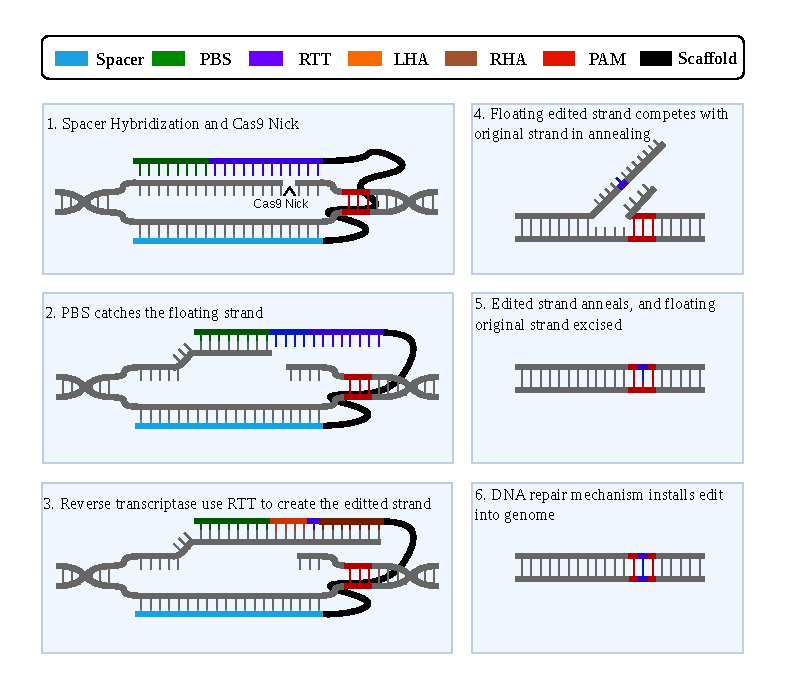
\includegraphics[width=0.95\linewidth]{diagrams/illustration/prime editing process.pdf}
    \caption{Prime editing components and mechanism~\cite{anzaloneSearchandreplaceGenomeEditing2019}.
    A prime editor (PE) fuses a Cas9 nickase with reverse transcriptase; both protein modules are omitted here for visual clarity.
    The prime editing guide RNA (pegRNA) contains a target-directing \textit{spacer}, a Cas9 \textit{scaffold}, a \textit{primer-binding site} (PBS), and a \textit{reverse-transcriptase template} (RTT) encoding the desired change as left homology arm (LHA), \textit{edit}, and right homology arm (RHA); the \textit{PAM} (red) enables target recognition and nicking.}
    \label{fig:pe-process}
\end{figure}


Together, these components install programmed sequence changes through a nick-and-copy mechanism~\cite{anzaloneSearchandreplaceGenomeEditing2019}.
After the prime editor--pegRNA complex binds the target locus and nicks the PAM-containing strand, the exposed 3$'$ end hybridizes to the PBS and primes reverse transcription of the RTT, copying the desired edit onto a newly synthesized 3$'$ flap (\autoref{fig:pe-process}, steps~1--3).
The subsequent steps are less deterministic.
Reverse transcription produces a branched intermediate in which the edited 3$'$ flap and the displaced original 5$'$ flap can equilibrate between competing annealing configurations (step~4).
Cellular flap-processing enzymes such as FEN1 preferentially excise the 5$'$ flap and ligate the edited strand when flap resolution favours the edit (step~5).
However, the outcome is not guaranteed: the edited flap may fail to invade the duplex, or 3$'$ exonucleases indigenous to the cell may degrade it, restoring the original sequence and leaving the target available for another round of editing from step~1~\cite{anzaloneSearchandreplaceGenomeEditing2019}.
Even when the edited strand is ligated, the resulting heteroduplex still contains mismatches between the edited and unedited strands that must be resolved by mismatch repair~(MMR) or replication (step~6).
Because MMR can use either strand as template, it may reject the edit, restore the original allele and reset the locus~\cite{anzaloneSearchandreplaceGenomeEditing2019,chenEnhancedPrimeEditing2021}.
These competing repair outcomes help explain why raw prime editing efficiencies are often modest, and they motivate enhanced systems such as PE3~\cite{anzaloneSearchandreplaceGenomeEditing2019}, which nicks the non-edited strand to bias heteroduplex resolution, and PE4/PE5, which transiently suppress MMR with a dominant-negative MLH1 protein~\cite{chenEnhancedPrimeEditing2021}.

On top of the competing repair outcomes, editing efficiency is also heavily shaped by target context and pegRNA design.
Cis-chromatin position effects and local epigenetic marks can strongly modulate prime editing even for a fixed pegRNA~\cite{liChromatinContextdependentRegulation2024,mathisMachineLearningPrediction2024}, but because these locus-level effects are largely separable from pegRNA sequence design and are typically modelled as a separate problem (e.g.\ ePRIDICT), chromatin context is not the focus of this study.
Instead, this work centres on sequence-level determinants of efficiency.
High-throughput analyses show that position-specific nucleotide composition in the target and pegRNA flanking regions---including PBS and reverse-transcriptase template (RTT) GC content, PAM choice, and the identity of the last templated nucleotide---can shift activity by orders of magnitude~\cite{kimPredictingEfficiencyPrime2021,kimChromatinStructureContextdependent2023}.
pegRNA architecture adds another layer of control: optimal primer-binding site (PBS) length depends on delivery format and on melting temperature of PBS--target hybridization, because complementarity between the PBS and spacer can auto-inhibit target binding~\cite{ponnienselvanReducingInherentAutoinhibitory2023}, and degradation of the 3$'$ RTT--PBS extension can poison editing unless the pegRNA is stabilized, for example with engineered 3$'$ RNA structures~\cite{nelsonEngineeredPegRNAsImprove2022}.
Nevertheless, many sequence determinants remain only partly understood.
For some edit classes, such as insertions, it remains unclear which sequence and repair features govern efficiency even after large-scale profiling~\cite{koeppelPredictionPrimeEditing2023}.
As a result, efficient prime editing often requires laborious empirical optimization rather than design from first principles~\cite{kimChromatinStructureContextdependent2023,domanDesigningExecutingPrime2022,hsuMechanisticMachineLearning2026}.
That combinatorial barrier matters because a therapeutic path is already in view.
Nuclease-based CRISPR-Cas9 has reached the clinic: exagamglogene autotemcel disrupts an enhancer of \textit{BCL11A} to reactivate foetal haemoglobin, with clinical benefit in severe sickle cell disease~\cite{frangoulExagamglogeneAutotemcelSevere2024}.
This is a compensatory edit, not a correction of the causal \textit{HBB} allele.
Prime editing can in principle install that correction---and, more broadly, the substitutions, insertions and deletions that gene disruption cannot---without double-strand breaks~\cite{anzaloneSearchandreplaceGenomeEditing2019,everetteExVivoPrime2023}.
Realising that potential still depends on choosing an efficient pegRNA from a large design space.

This motivates computational tools for in silico pegRNA design given a target sequence and a desired edit.
Such tools generally operate in two stages.
First, candidate pegRNAs are proposed from physical constraints such as PAM availability and limits on PBS and RTT length; most pipelines follow similar principles here.
The second, more consequential stage ranks those candidates with a model trained on experimental efficiency data.
Three major model families have emerged---conventional machine learning~\cite{liEasyPrimeMachineLearning2021,koeppelPredictionPrimeEditing2023}, deep learning~\cite{kimPredictingEfficiencyPrime2021,yuPredictionEfficienciesDiverse2023,schwankgeraldPredictingPrimeEditing2023,mathisMachineLearningPrediction2024}, and mechanistic models~\cite{hsuMechanisticMachineLearning2026}---each with distinct strengths and limitations.
Yet these models are trained and released on heterogeneous datasets, input formats, and evaluation protocols, which makes fair comparison difficult and leaves little shared infrastructure for combining complementary predictors.

To address this gap, I present a prime editing benchmarking platform that unifies large-scale experimental datasets under a common schema, evaluates state-of-the-art efficiency predictors side by side, and supports training custom models as well as ensembles that mix newly trained weights with vendor-provided ones.

\section{Methods}

\subsection{Project Structure Overview}

The platform comprises two Python FastAPI services and a shared web interface. PE Database (PE-DB) owns the experimental-data catalog, standardization, filtering, and conversion to model-specific inputs. PE Ensemble owns model loading, training, hyperparameter search, evaluation, and prediction combination. PE Hub provides a React/TypeScript interface to both services. A shared Python package, \nolinkurl{pe-common}, implements sequence utilities, target identifiers, data splitting, regression metrics, and training helpers so that the services use the same definitions. Both backends also expose in-process Python libraries and command-line interfaces, allowing the same workflows to run without HTTP servers.

\subsection{PE Database}
% overview of the database operations

Large-scale prime editing studies have produced a growing body of data, but differences in input formats and experimental annotations leave their usage with substantial overhead. PE-DB was developed to make these datasets accessible through a common representation, and brings together guide RNA sequences, target DNA sequences, and measured editing outcomes from these experiments.

PE-DB focuses on datasets suitable for training and benchmarking efficiency predictors. Small datasets from studies of specific prime editing systems, such as Nelson et al.\cite{nelsonEngineeredPegRNAsImprove2022}, are therefore not included in this project.

However, widely used validation datasets such as Anzalone et al.\cite{anzaloneSearchandreplaceGenomeEditing2019} are retained despite their small size because they are frequently used to validate published prediction models.

\subsubsection{Data Source}

The database brings together six large-scale studies spanning several prime editor variants, cell lines, and experimental settings, plus the Anzalone et al.\ 2019 endogenous validation set:

\begin{enumerate}
    \item \textbf{Anzalone et al. 2019}

    Anzalone et al.\cite{anzaloneSearchandreplaceGenomeEditing2019} introduced prime editing and reported arrayed PE2/PE3 efficiencies at a small number of endogenous genomic loci (primarily HEK293T). It remains a standard external validation resource for published predictors (Easy-Prime, PRIDICT, DeepPrime, among others) despite its small size. PE-DB stores the Li et al.\ (Easy-Prime) reformatting of those experiments as \nolinkurl{anzalone-endo}: replicate-averaged HEK293T PE2 ($n = 199$) and PE3 ($n = 278$) pegRNAs. Standardization expands each design onto a sense-oriented hg38 window large enough for vendor protocols: DeepPrime crops a real 74\,bp PE-core layout from the Easy-Prime amplicon (no 3$'$ \texttt{N} pad), and OPED receives Liu's 350\,bp BLAT-style window (165\,bp upstream of the spacer + 20 + 165\,bp down) cached from local hg38 spacer matches.

    \item \textbf{Kim et al. 2021}

    Kim et al.\cite{kimPredictingEfficiencyPrime2021} conducted one of the first big-data studies on prime editing efficiency, performing a high-throughput evaluation of PE2 activity using 54,836 pairs of pegRNAs and target sequences in HEK293T cells. The study identified factors affecting PE2 efficiency and developed three computational models (including the deep learning model DeepPE) to predict pegRNA efficiency. The data are organized into four datasets in the database from their original two libraries.

    The main library \nolinkurl{deeppe-ht} contains approximately 43,000 pegRNAs from  library~1, which focused on a G$\to$C substitution at reverse transcriptase template position +5. These pegRNAs and their corresponding synthetic target sequences were delivered via lentiviral reporters --- each construct pairs the pegRNA with an artificial target cassette rather than an endogenous genomic locus.

    Library~2 is split into an edit-type subset \nolinkurl{deeppe-type}, which evaluates how different mutation types (substitutions, insertions, deletions) affect PE2 efficiency, and an edit-position subset \nolinkurl{deeppe-position}, which evaluates how the position of the edit within the reverse transcriptase template affects efficiency. Both subsets use the same lentiviral reporter system in HEK293T cells with PE2.
    The exported HEK293T--PE2 sheets contain 4{,}178 rows in \nolinkurl{deeppe-type} and 1{,}974 in \nolinkurl{deeppe-position}; \nolinkurl{deeppe-ht} contains 43{,}149 rows, after removing entries without a numeric efficiency measurement.

    A separate endogenous validation dataset \nolinkurl{deeppe-endo} contains arrayed pegRNA experiments at native genomic loci in HEK293T, HCT116, and MDA-MB-231 cells, where both pegRNAs and PE2 were delivered by plasmid transfection. Editing efficiencies are averaged across biological and technical replicates (BR1--BR2 $\times$ TR1--TR2).

    \item \textbf{Yu et al. 2023}

    As a follow-up study to Kim et al. 2021, Yu et al.\cite{yuPredictionEfficienciesDiverse2023} systematically evaluated prime editing efficiencies for a much larger number of pegRNA--target pairs (338,996 pegRNA--target pairs, including 3,979 epegRNAs) in an error-free manner across eight PE systems and seven cell types.

    The main ClinVar library \nolinkurl{deepprime-clinvar} contains approximately 259,000 pegRNA--target pairs designed around ClinVar pathogenic variants. Efficiencies were measured on synthetic 74~bp target contexts via a plasmid-based assay similar to Kim et al. 2021. 

    The fine-tuning datasets \nolinkurl{deepprime-small} are smaller datasets that span multiple PE systems (PE2, PE2max, PE4max, NRCH-PE2, NRCH-PE2max, NRCH-PE4max, among others) and cell types (HEK293T, A549, DLD1, HeLa, MDA-MB-231, HCT116, and NIH3T3).

    Two off-target datasets are also stored in the database: a mismatch library \nolinkurl{deepprime-off} and its sub-pools \nolinkurl{deepprime-off-subpool}, which profile PE editing efficiencies at mismatched target sites.

    \item \textbf{Koeppel et al. 2023}

    Koeppel et al.\cite{koeppelPredictionPrimeEditing2023} focused specifically on prime editing insertion efficiency, designing a library of 3,604 insertion sequences of various lengths (1--69~nt) and measuring their insertion frequencies at four endogenous genomic target sites (HEK3, EMX1, FANCF, and the safe-harbor CLYBL locus) in three human cell lines (HEK293T, HAP1, and HAP1 $\Delta$MLH1). 

    MinsePIE data are split into five catalog datasets by library design and delivery:
    \nolinkurl{library-insert-set12} (Set~1/2 pooled screens),
    \nolinkurl{library-insert-18nt} (18~nt insertion library),
    \nolinkurl{library-insert-codon-variant} (endogenous barnacle tagging),
    \nolinkurl{library-insert-codon-hek3} (codon validation at HEK3), and
    \nolinkurl{library-insert-piggybac} (Set~1 screens in HAP1 with PiggyBac-integrated PE2).
    Only 19 out of 33 sets of experimental data from the study were recorded into the database, as the experimental results for the additional validation experiments could not be located.

    \item \textbf{Schwank et al. 2023}

    Schwank et al.\cite{schwankgeraldPredictingPrimeEditing2023} performed a high-throughput screen analyzing prime editing outcomes of 92,423 pegRNAs targeting a highly diverse set of 13,349 human pathogenic mutations, including base substitutions, insertions, and deletions.

    The main library \nolinkurl{library1} uses a self-targeting lentiviral reporter format in HEK293T cells that is also similar to Kim et al. 2021. The pegRNAs were delivered by lentiviral transduction and PE2 was delivered by plasmid transfection.

    The secondary dataset \nolinkurl{library2} is a disease-focused subscreen of the same lentiviral reporter format across HEK293T, U2OS, and K562 (with and without MMR inhibition by co-transfecting dominant-negative MLH1). The library2-invivo dataset validates the same pegRNA set in GFP+ sorted mouse liver via adenoviral delivery of both pegRNAs and PE2.

    A separate endogenous validation dataset \nolinkurl{pridict1-endo} contains arrayed pegRNA experiments at 15 genomic loci in HEK293T and K562 (three pegRNAs per locus from library~1: the endogenous-target pegRNA, \emph{endo}, plus the highest- and lowest-PRIDICT-scoring candidates, \emph{best} and \emph{worst}). Edit types are taken from the authors' endogenous CRISPResso batch amplicons (PRIDICT supplementary files): 44 pegRNAs install a 1-bp substitution and locus~3 uses a 10-bp deletion; there are no insertion edits in this validation set.

    \item \textbf{Mathis et al. 2024}

    The library-diverse dataset extends the PRIDICT1 approach with a broader range of edit types, screened in HEK293T, K562, and K562 with co-transfected dominant-negative MLH1 (MLH1dn) using the same self-targeting lentiviral reporter system, with the same delivery method as PRIDICT1.

    The library-diverse-invivo dataset validates a subset of the diverse-library pegRNAs at endogenous mouse liver loci in vivo, where both pegRNAs and PE were delivered via adenoviral vectors. This provides an important cross-context validation for computational predictions trained on in vitro reporter data.

    Additionally, a TRIP (Thousands of Reporters Integrated in Parallel) analysis dataset profiles editing at 1,202 endogenous genomic integration sites in K562 cells, providing the chromatin context data used to train their ePRIDICT model. Every integration was edited with the same prime-editing pegRNA (\nolinkurl{TRIP\_pegRNA\_GtoC}), a uniform 1-bp G$\to$C substitution. 

    \item \textbf{Hsu et al. 2026}

    Hsu et al.\cite{hsuMechanisticMachineLearning2026}  performed two large paired pegRNA--target lentiviral reporter screens in HEK293T (partially mismatch-repair deficient) and HeLa (mismatch-repair proficient) cells, measuring editing with both PE2 and PE4. In both screens, pegRNA--target pairs were packaged into lentiviral libraries and transduced at low multiplicity of infection (MOI~$<0.3$); after selection for integrated library members, cells were transfected with PE construct plasmids (PEmax) to induce editing.

    The \nolinkurl{lib-mmr} library  comprises ${\sim}$9,964 pegRNAs targeting 200 randomly selected exonic sites with diverse edit types, including single and multi-base substitutions, insertions, deletions, and PAM edits. The supplementary table also lists 36 additional pegRNAs with \nolinkurl{Design category = Endogenous}; these are positive controls whose sequences were previously used to edit endogenous loci (RNF2, FANCF, HEK3, APOE, HBB, CDKL5, PRNP, and HEXA), but in this study they were assayed in the same lentiviral reporter format as the rest of Lib-MMR, not to be confused with the endogenous edits performed in the studies like MinsePIE. PE DB stores them separately as \nolinkurl{lib-mmr-controls} so that users can include or exclude reference pegRNAs without mixing them into the primary MMR diversity library.

    The \nolinkurl{lib-cv} library contains 10,406 pegRNAs designed to correct 944 ClinVar pathogenic variants, including up to nine silent edit combinations per variant to evade mismatch repair.     Like Lib-MMR, Lib-CV uses the lentiviral pegRNA--target reporter system with PE2/PE4 plasmid transfection in HEK293T and HeLa. Across the two libraries, the authors report 74,769 editing measurements spanning 1,290 unique target sites in these four cell-line/PE-system combinations. 

\end{enumerate}

\begin{figure}[ht]
    \centering
    \includegraphics[width=\linewidth]{diagrams/data_composition.png}
    \caption{Composition of the data from the studies. \textbf{A.} Edit length (log scale). \textbf{B.} Edit type: `sub' substitutions, `ins' insertions, `del' deletions. \textbf{C.} Edit scope: off-target designs use a pegRNA against a non-matching target. \textbf{D.} Experimental method. \textbf{E.} Target context. \textbf{F.} pegRNA delivery. \textbf{G.} PE delivery. Bars are stacked by source study.}
    \label{fig:data_composition}
\end{figure}

\autoref{fig:data_composition} summarizes the catalogued measurements: 756,341 pegRNA--target pairs across seven studies. About two-thirds of designs install a 1~bp edit (512,055; panel~A), and substitutions dominate the collection (451,156), followed by insertions (202,663) and deletions (102,522; panel~B). DeepPrime and PRIDICT2 cover all three edit types. PRIDICT2 includes edits of 1--15~bp, compared with 1--3~bp in the main DeepPrime library and up to 6~bp in its fine-tuning subsets. Longer events, including an 18-nt insertion library and insertions of up to 69~bp, come almost entirely from MinsePIE.

The remaining panels show how these measurements were collected. Nearly all pairs are on-target (720,421 versus 35,920 off-target mismatch reporters from DeepPrime; panel~C) and were assayed in vitro (736,786 versus 19,555 in vivo mouse-liver measurements from the PRIDICT studies; panel~D). Endogenous chromosomal contexts account for 61,941 pairs, against 694,400 synthetic reporter designs (panel~E). pegRNAs were delivered mainly by plasmid transfection (395,096) or lentivirus (341,690); the in vivo subset used adenovirus (19,555; panel~F). The prime editor itself is almost always transfected as plasmid (723,516); the remainder are adenoviral (19,555) or PiggyBac-integrated PE2 in HAP1 (13,270; panel~G).


\subsubsection{Data Storage}

Since the project is distributed using GitHub, we needed to work around the 100 MB per file limit to avoid using Git LFS(Large File Storage) and incurring substantial charges.
The original TSV, CSV, and XLSX files are retained as source data. When PE-DB is initialized, these files are exported into experiment-specific CSV tables and standardized as Parquet files. A persistent SQLite catalog stores the associated metadata and file paths, while individual editing measurements are loaded from the tables as needed.

Usage of DVC is recommended for storing and synchronizing experimental data alongside `rsync', especially when working on clusters as they offer storage that can be used for DVC store. It would require you to create a new fork of this project since it needs to work with git, but the ability to version control the training and evaluation data is a great advantage. An example of setting up DVC to work on Oxford ARC Cluster has been provided in \nolinkurl{scripts/cluster/oxford-arc/setup_dvc_remote.sh}.

\subsubsection{Data Formatting}

The source studies use different file layouts, sequence conventions, and measurement columns. A common preprocessing pipeline makes these data usable across models.

First, each source file is divided into experiment-level tables, termed \textbf{datasheets}, each representing one PE system editing one cell line in one experiment setting. This export stage preserves the original columns wherever possible; sequence reconstruction and feature conversion are handled separately.

The shared \textbf{PE-core} format provides an intermediate representation between the source tables and the inputs required by each model. Study-specific exporters and standardizers construct PE-core records from the deposited tables; a separate converter for each supported model then recreates its native inputs from PE-core. This separates source-study reconstruction from model feature engineering, so adding a model does not require a new converter for every study.

The shared PE-core schema for library studies using synthetic reporter cassettes (Kim et al. 2021 deeppe-ht, Schwank et al. 2023 pridict library 1, 2, Mathis et al. 2024 library-diverse etc.) stores:
\begin{itemize}
    \item a protospacer-based group identifier (\nolinkurl{group\_id}) and the wild-type and mutated target-strand sequences (\nolinkurl{wt\_sequence}, \nolinkurl{mut\_sequence}),
    \item mutually exclusive substitution/insertion/deletion flags (\nolinkurl{type\_sub}, \nolinkurl{type\_ins}, \nolinkurl{type\_del}),
    \item edit length (the span from the first to the last base for multi-base substitutions) (\nolinkurl{edit\_len}),
    \item 0-based half-open geometry for the protospacer (\nolinkurl{protospacer\_location\_l}/\nolinkurl{\_r}), PBS (\nolinkurl{pbs\_location\_l}/\nolinkurl{\_r}), reverse-transcriptase template (\nolinkurl{rtt\_location\_l}/\nolinkurl{\_r}), and homology arms (\nolinkurl{lha\_location\_l}/\nolinkurl{\_r}, \nolinkurl{rha\_location\_l}/\nolinkurl{\_r}),
    \item optional DeepSpCas9 score (\nolinkurl{spcas9\_score}),
    \item measured editing efficiency (\nolinkurl{editing\_efficiency}), and
    \item optional author fold identifier if the authors explain the data split in any part of the study (\nolinkurl{original\_fold}).
\end{itemize}

Endogenous sheets use the same PE-core columns, but with additional columns for the genomic coordinates and the reference window. When a genomic reference window can be cached, the aligned WT/Mut pair is embedded in a target-strand context sized for the study: the shared endo PE-core uses 200~bp with the 20-nt protospacer at offset 90, while Anzalone OPED evaluation expands to Liu's 350~bp layout (spacer at offset 165) to match their protocol. Those windows are large enough that later DeepPrime and PRIDICT crops do not have to invent 3$'$ DNA, and OPED can consume the full available WT without padding. Eight nullable \nolinkurl{endo\_*} columns record assembly, chromosome, a 0-based half-open genomic interval (typically the protospacer), strand, what the interval anchors, a provenance string, and an optional locus label. Gene, chromatin, and expression annotations are not stored, since they can be recovered later from coordinates and cell-line context.

For PRIDICT1 \nolinkurl{library2-invivo}, coordinates and reference windows are both keyed by variant \nolinkurl{Name}. The sheet has 179 unique Names, and 167 of them are placed on hg38 or mm39. Human ClinVar HGVS names are placed with Ensembl VEP. Every other human Name needs a unique exact match of its deposited protospacer on local hg38, and each mouse ortholog needs the same match on local mm39. Twelve Names stay unplaced. Eight are ribosomal-protein edits (\nolinkurl{RPL}/\nolinkurl{RPS}) whose 20-nt protospacer is not a unique hg38 hit: the column adds a non-genomic 5$'$ G in front of the 19~nt cassette spacer, and several of these sequences occur at more than one locus. Four are mouse orthologs with no unique hit in the local mm39 FASTAs, which contain only chr10 and chrX. One further mouse Name does match chr10 and is counted among the 167.

A 200~bp window is cached for a placed Name only when that 19~nt cassette spacer exact-matches the reference interval. This succeeds for 77 of the 167 Names. The other placed Names keep coordinates and no window, usually because a ClinVar spacer carries the pathogenic allele and so is not the reference sequence. The loci table stores one window per Name, while 110 Names are measured with two or three different spacers. At standardization a row is embedded in the cached window only when its own spacer matches that window to within two bases. Every other row keeps the author 99~bp cassette.

MinsePIE requires additional reconstruction steps. Koeppel et al. reported insertion efficiencies at endogenous loci, but the supplementary tables identify each target only by a short name (HEK3, EMX1, FANCF, CLYBL, and so on) together with the pegRNA spacer, PBS, and homology-arm (HA) sequences from Supplementary Table~6 (ST6). No genomic coordinates or extended wild-type context windows are provided, so the wide target-strand sequences required by the shared PE schema must be reconstructed.

During exportation, each MOESM5 experiment string is mapped to the corresponding ST6 pegRNA row so that spacer, PBS, HA, and annotated insertion position (\texttt{+N}) are attached to every measured insert. Where the HA encodes a non-\texttt{+1} insertion, an \texttt{-Ins-} marker splits the RTT-oriented HA into left and right segments; on the target strand these become the reverse complements of HA-right (immediately 3$'$ of the SpCas9 nick between protospacer positions 17 and 18) and HA-left (further 3$'$ of the insertion).

The genomic anchors themselves were obtained by exact (and reverse-complement) mapping of the ST6 spacers onto GRCh38/hg38, since many author supplied location names are not conventional genomic sites. Classic PE-site coordinates cited elsewhere in the literature were checked and discarded when they did not contain the MinsePIE spacer: in particular, the HEK3 site used throughout the study maps to \textit{LINC01509} on chromosome~9 rather than the chromosome~11 locus often associated with HEK293 editing screens. For the 18-nt library, the Methods text places HEK3-S2--S6 within approximately 1~kb of that HEK3 anchor as per author's description; sites that differed from the reference by a single base (HEK3-S3/S5/S6 and some codon-variant pegRNAs) were placed by homology-arm context and the flanking sequence was patched so that the ST6 spacer sits at a fixed 90~bp offset within a 200~bp flank. The resulting loci table (\nolinkurl{MinsePIE\_genomic\_loci.json}) stores chromosome, 1-based spacer start, assembly strand, and the reference window for each of the 17 ST6 targets. Standardization then inserts the measured sequence at the nick/HA-derived edit position to produce length-matched WT (N-padded at the insertion) and Mut sequences on that 200~bp window, and records the corresponding hg38 protospacer interval.

However, not every endogenous measurement can be placed in the extended PE-core format, some data remain catalogued but are excluded from conversion to the full PE-core standardized tables.

The PRIDICT1 arrayed endogenous table (\nolinkurl{endogenous}) reports locus-level efficiencies and chromatin marks without pegRNA-linked WT/Mut sequences or geometry, so it is stored as a filter-only (partial) sheet. PRIDICT2 TRIP (\nolinkurl{trip-analysis}) records barcode, hg38 integration coordinate, and efficiency for 1{,}202 sites edited with the same G$\to$C pegRNA, but the deposited table does not include the pegRNA sequences; support for TRIP data is therefore also partial: integration coordinates are attached, but model-format export is disabled until the pegRNA can be reconstructed.

PRIDICT2 \nolinkurl{library-diverse-invivo} is another special case. It reports endogenous editing efficiencies in mouse liver, but is standardized in the plain PE-core library schema without genomic coordinates or reference windows. The deposited 99~bp target contexts are already long enough for the supported model converters, and unlike MinsePIE---which required spacer mapping onto a handful of named loci to recover missing WT/Mut sequence---this sheet provides no locus anchors for ${\sim}$10{,}700 unique spacers across ${\sim}$18{,}000 measurements, making genome-wide placement impractical at that scale.

\subsubsection{Model-specific Feature Construction}

From PE-core, PE-DB is capable of constructing the input features for each supported model. 

DeepPrime receives a 74-base wild-type window with the protospacer starting at offset four, a masked 74-base edited representation containing the PBS and RTT, and its engineered sequence features. These include lengths, edit indicators, GC composition, melting temperatures, RNA minimum free energies, and the DeepSpCas9 score. 

OPED receives the full unpadded wild-type target already present on the standardized row (DeepPE reporters remain 47~bp; endogenous Anzalone rows expanded to Liu's 350~bp hg38 window, while all other datasets use as much of the target context as possible), a PBS extracted from the wild-type sequence, and an RT sequence extracted from the mutant sequence. 

The PRIDICT2 conversion pipeline starts by constructing initial and mutated target sequences, edit positions and lengths, region annotations, with the spacer at offset ten. Followed by thermodynamic features, including seven ViennaRNA minimum-free-energy features for the spacer, scaffold, PBS, RT, and their combinations. 

OptiPrime receives the spacer and reverse-complemented PBS and RTT in the RNA alphabet, together with unedited and edited DNA contexts aligned to Hsu's four-base upstream protospacer frame (short reporter windows without upstream sequence are left-padded with \texttt{A}). Assay metadata---scaffold, epegRNA motif, Cas9 variant, PE type, integration time, and kinetic \texttt{group}---are set from the source study and cell line so that trained group factors load correctly to adjust the scale of the editing efficiency measurement.

Where the source lacks sufficient flanking sequence, conversion follows model-specific conventions rather than inventing DNA for OPED: DeepPrime uses \texttt{N} for missing target context and \texttt{X} for masked edited positions when a 74~bp window cannot be filled from the source. OPED simply passes through whatever unpadded WT length is available as the transformer architecture is designed to handle variable length inputs.

Converted frames are cached on disk with a converter revision check to avoid repeating expensive feature calculations. Missing or non-numeric efficiency labels are removed during standardization, and model training rejects missing labels that reach a wrapper through an alternative input path.

\subsubsection{Database Design}

The catalog uses a hierarchical schema to separate publication-level information from experiment-specific metadata. Shared annotations are stored once at the appropriate level and inherited through the table relationships, reducing duplication while supporting detailed filtering.

\begin{figure}[ht]
    \centering
    
\includegraphics[width=0.95\textwidth]{diagrams/illustration/database_er.png}
    \caption{ER diagram of the implemented PE-DB catalog schema (\nolinkurl{study}, \nolinkurl{dataset}, \nolinkurl{scaffold}, \nolinkurl{datasheet})}
    \label{fig:database_er}
\end{figure}

As shown in \autoref{fig:database_er}, the implemented catalog schema consists of four relational tables: \textbf{Study}, \textbf{Dataset}, \textbf{Scaffold}, and \textbf{Datasheet}.

The \textbf{Study} table represents the publication level of the hierarchy and stores one row per source study. It contains a unique study name, optional publication date, and optional author string. Each study is linked to one or more datasets through a one-to-many relation.

The \textbf{Dataset} table forms the intermediate layer and stores dataset-level metadata shared across many experiments. Implemented fields include dataset name, optional textual description, pegRNA delivery method, PE delivery method, edit scope, experimental method, target context, and the \nolinkurl{standardizable} flag. \nolinkurl{standardizable=True} means full conversion support to the shared standardized format, while \nolinkurl{standardizable=False} means partial support (entry-level fields only, for example PRIDICT2 TRIP dataset). A foreign key (\nolinkurl{study\_id}) links each dataset to its parent study.

The \textbf{Scaffold} table stores pegRNA scaffold definitions as reusable reference records. Each scaffold has an explicit identifier, scaffold name, sequence, and optional description. This separates scaffold metadata from experiment-specific metadata and allows many datasheets to reuse the same scaffold entry.

The experiment level is represented by the \textbf{Datasheet} table. Each datasheet points to one exported CSV file containing the data of one PE system targeting a specific cell line under the experimental condition specified in the \textbf{Dataset} table, and stores the additional metadata required by the API: file path, cell line, PE system, scaffold, number of samples, and an \nolinkurl{updated\_at} timestamp. Foreign keys (\nolinkurl{dataset\_id} and \nolinkurl{scaffold\_id}) connect each datasheet to both its parent dataset and scaffold record.

The catalog contains the metadata needed to select experiments, while individual editing measurements remain in separate files. The catalog stores paths to the exported experiment tables, with standardized Parquet files used for filtering and model-format conversion. This keeps the relational catalog small and defers loading the larger measurement tables until they are needed. Filters on individual edits are only applied to the datasheets that meet the requested experimental conditions.

\subsubsection{Filtering for well-designed pegRNAs}
Hsu et al. \cite{hsuMechanisticMachineLearning2026} pointed out that existing datasets contain a large number of poorly designed pegRNAs that would never be used in practice by experienced technicians, thus the performance of existing models trained and benchmarked on these datasets is not representative of the real world performance and is potentially inflated with easily identifiable features that lead to poor editing efficiency.

PE-DB therefore includes optional design rules that users can apply before export or evaluation.

Two named rulesets are available as \nolinkurl{--design-ruleset} (also on \nolinkurl{peen evaluate}):

\begin{itemize}
    \item \textbf{\nolinkurl{optiprime}} (alias \nolinkurl{hsu}) --- Hsu et al.\ ~'s library construction constraints that the deposited libraries follow consistently: PBS length 13; first nucleotide of the pegRNA reverse-transcriptase template is not C. Hsu's Methods also prescribe 3$'$ homology of $9+L$ (substitutions) or $19+L$ (insertions and deletions), then a length nudge so the first RTT base is not C; that clause is implemented as the optional atomic rule \nolinkurl{homology\_hsu} but is \emph{not} part of the named preset (see Results).
    \item \textbf{\nolinkurl{anzalone}} --- Anzalone et al.\ (2019) stated these design guidelines in their study introducing prime editors: PBS 10--16\,nt, PBS GC content 40--60\%, RTT 10--16\,nt, and first RTT nucleotide not C.
\end{itemize}

Atomic rules are also available (\nolinkurl{pbs\_13}, \nolinkurl{rtt\_not\_c}, \nolinkurl{homology\_hsu}, \ldots) and can be selected individually, and multiple names can be combined with AND. 
% The unfiltered evaluation remains the default; repeating the base-model matrix with \nolinkurl{DESIGN\_RULESET=optiprime} scores only the well-designed subset.

\subsubsection{Data Retrieval and Interaction}

PE-DB exposes the same catalog and filtering operations through two entry points that share one headless library (\nolinkurl{pe\_db.library}): a FastAPI HTTP service and the \nolinkurl{pedb} command-line interface. The web portal and PE Ensemble's HTTP path use the FastAPI routes, while \nolinkurl{pedb} and the \nolinkurl{peen} CLI call the library directly so batch jobs need no running PE-DB server.

The FastAPI app provides endpoints for browsing studies, datasets, datasheets, and scaffolds, retrieving summary statistics, and filtering experimental records. The \nolinkurl{pedb} CLI mirrors those query operations (\nolinkurl{pedb studies}, \nolinkurl{datasets}, \nolinkurl{datasheets}, \nolinkurl{scaffolds}, \nolinkurl{statistics}, \nolinkurl{filter}, \nolinkurl{formats}) and additionally covers administrative pipeline steps that are not exposed as HTTP routes---catalog seeding, raw export, standardization, single-sheet conversion, plugin reload, and formatted-cache clearing (\nolinkurl{pedb init}, \nolinkurl{export}, \nolinkurl{standardize}, \nolinkurl{convert}, and related commands).

The shared filter path (\nolinkurl{GET /api/filter} and \nolinkurl{pedb filter}) first selects experiments by their catalog metadata, then applies row-level constraints such as edit type, edit length, and design rules. The resulting records can be returned in PE-core or converted to a supported model format. Partial datasets remain available for exploration, but model-format requests skip tables that lack the required sequence information and report the reason.

PE-DB's filter function also assigns partitions before the model wrapper receives its input. Supported strategies are a two-way train/test holdout, a three-way train/validation/test holdout, and grouped cross-validation with an optional separate test holdout. Synthetic partitions shuffle target groups with a configurable random seed (default 42), so pegRNAs sharing a protospacer remain together. When datasheets are explicitly merged, group identifiers are reassigned from protospacer sequences across the merged collection before splitting. Author-provided partitions can be selected through \nolinkurl{original_fold}; the default request asks for an 80/20 holdout while preferring author folds, with $-1$ as the default author test identifier (a different identifier can select a PRIDICT2 held-out run). Author-fold assignments take precedence over synthetic fractions if user is requesting to use author-provided partitions.

Although the ability to join sheets from different studies is implemented, it is not always sensible to do so. The editing efficiency measurement produced by different studies under different experimental conditions is often not directly comparable on the same scale\cite{schwankgeraldPredictingPrimeEditing2023}.
The studies also differ in how they report editing efficiency. Kim et al. set the standard of using the augmented editing efficiency measurement, which deducts the background editing rate from the total editing rate, for all of their datasets\cite{kimPredictingEfficiencyPrime2021,yuPredictionEfficienciesDiverse2023}. The background editing rate is the editing rate of the pegRNA in the absence of the target sequence, measured in 0-100 scale, thus the $\div 100$ in \autoref{eq:augmented-editing-efficiency}. This measurement method is also followed by the PRIDICT studies\cite{schwankgeraldPredictingPrimeEditing2023,mathisMachineLearningPrediction2024}. Koeppel et al., however, used the ratio of successful insertions over total insertions as the editing efficiency measurement. The background editing rate was not provided in the study and thus currently impossible to recover; this difference in label definition may contribute to differences in model performance across datasets. 

% PRIDICT1 has the maximum flexibility by providing the raw counts for intended edits, unintended edits, and unedited reads. 

\begin{equation}
    \text{Editing efficiency} = 100 \times \frac{\text{\# successful edits} - \text{\# total read count} \times \text{background editing rate} \div 100}{\text{\# total read count} - \text{\# total read count} \times \text{background editing rate} \div 100}
    \label{eq:augmented-editing-efficiency}
\end{equation}

\subsection{PE Ensemble}

PE Ensemble builds on PE-DB to support model benchmarking, retraining, and the evaluation of custom ensembles.

For each job, PE Ensemble requests the selected experiments data in the format registered for the model from PE-DB, resolves a named weight set or training configuration, and calls a common model-wrapper interface. This allows the same data selection to be reused across architectures while retaining their native preprocessing and inference routines.

Similar to PE-DB, these operations are available through the web interface, API, and command line.

\subsubsection{Models}
\label{subsubsection:models}

The benchmark includes predictors that score substitutions, insertions, and deletions, so the same pegRNA--target table can be evaluated under every model. MinsePIE\cite{koeppelPredictionPrimeEditing2023} falls outside that scope: it estimates insertion frequency only, and it reports the ratio of successful insertions to total insertions, a different label from the background-subtracted efficiency used by the other studies. 

Within each lineage, the later model is the one included. DeepPrime\cite{yuPredictionEfficienciesDiverse2023} is the later model from the DeepPE group\cite{kimPredictingEfficiencyPrime2021}: it is trained on the ClinVar screen, covers all three edit types up to 3~bp, and provides fine-tunes for cell line and PE system. PRIDICT2\cite{mathisMachineLearningPrediction2024} is the later model from the PRIDICT group\cite{schwankgeraldPredictingPrimeEditing2023}: it uses attention-based bidirectional RNNs, extends edits to 15~bp, separates mismatch-repair contexts, and reports higher correlation than PRIDICT~v1 on the screens both models score. 

These criteria leave three sequence models of different architecture---the OPED transformer\cite{liuDesignPrimeeditingGuide2023}, DeepPrime's convolutional--recurrent network, and the PRIDICT2 recurrent network with attention---and OptiPrime\cite{hsuMechanisticMachineLearning2026}, which obtains efficiency by integrating a prime-editing reaction scheme.

\begin{enumerate}
    \item \textbf{DeepPrime}

    Yu et al.\cite{yuPredictionEfficienciesDiverse2023} developed DeepPrime as a hybrid convolutional and recurrent architecture that encodes inter-sequence features between the target DNA and pegRNA. One-hot target--pegRNA tensors are processed by a 2D/1D CNN stack followed by a bidirectional GRU, while 24 engineered sequence features (for example GC content, melting temperatures, and minimum folding energies) are passed through a multilayer perceptron; the two representations are concatenated to predict editing efficiency. The model was trained on ClinVar\_Train ($n = 259{,}910$), the training split of the 288{,}793-pair ClinVar library, allowing the model to generalize across substitutions, insertions, and deletions of up to 3~bp. The same study also introduced DeepPrime-FT, which fine-tunes the base model to 18 cell-line and PE-system combinations across seven cell types and eight PE variants.
    
    On the held-out ClinVar test set ($n = 28{,}883$), DeepPrime achieved Pearson $r = 0.84$ and Spearman $R = 0.86$; performance remained high across nine edit-type subsets ($r = 0.76$--$0.89$, median $0.81$; $R = 0.70$--$0.88$, median $0.83$). 

    \item \textbf{PRIDICTv2}

    Mathis et al.\cite{mathisMachineLearningPrediction2024} extended the original PRIDICT framework with PRIDICT2.0, an ensemble of attention-based bidirectional recurrent neural networks. The model averages predictions from two components: one pretrained on PRIDICT library~1 and fine-tuned on the Library-Diverse screen, and another pretrained on the library~1 concatenated with DeepPrime ClinVar library before fine-tuning on Library-Diverse. Dual RNN encoders with attention layers process the wild-type and edited target sequence contexts separately, enabling predictions for substitutions, insertions, and deletions of up to 15~bp in mismatch-repair-deficient HEK293T, mismatch-repair-proficient K562, and K562 with co-transfected MLH1dn, as well as in vivo in mouse liver. 
    
    In grouped fivefold cross-validation on Library-Diverse, PRIDICT2.0 reached Spearman $R = 0.91$ / Pearson $r = 0.90$ in HEK293T and $R = 0.81$ / $r = 0.70$ in K562, outperforming PRIDICT~v1 on the same screens ($R = 0.83$ and $0.64$, respectively); gains were largest in K562 and for multi-base replacements and deletions.  Relative to PRIDICT~v1 ($R = 0.85$ / $r = 0.86$ on its 92{,}423-pegRNA Library~1)\cite{schwankgeraldPredictingPrimeEditing2023}, PRIDICT2.0 further generalized to longer edits and additional contexts. On endogenous and external sets it matched or exceeded PRIDICT~v1 (Mathis endogenous: HEK $R/r = 0.80/0.66$ vs.\ $0.81/0.69$, K562 $0.85/0.61$ vs.\ $0.69/0.48$; Anzalone HEK: $0.69/0.63$ vs.\ $0.47/0.47$).

    \item \textbf{OPED}
    
    Liu et al.\cite{liuDesignPrimeeditingGuide2023} developed Optimized Prime Editing Design (OPED), an interpretable nucleotide language model that applies transfer learning to pegRNA efficiency prediction. A transformer encoder extracts features from the target sequence, while custom transformer decoders model the PBS and RT template sequences and their cross-sequence dependencies; attention weights provide post-hoc interpretability of individual nucleotide contributions. OPED was initially trained on the DeepPE high-throughput training set, then fine-tuned and validated on three held-out DeepPE subsets. 

    On the HT-test, Type-test, and Position-test sets ($n = 4{,}457$, 403, and 200, respectively), OPED achieved Pearson $r = 0.769$, 0.612, and 0.628 and Spearman $R = 0.798$, 0.624, and 0.562; pegRNAs with higher predicted scores showed 8.0-, 3.1-, and 2.2-fold higher measured editing efficiencies. When retrained on the PRIDICT library~1 using their own training and validation splits, OPED reported $r = 0.912$ and $R = 0.905$ for editing efficiency and $r = 0.810$ and $R = 0.826$ for unintended editing rates on the test set ($n = 18{,}485$), consistently outperforming DeepPE, Easy-Prime, and PRIDICT. 

    \item \textbf{OptiPrime}

    Hsu et al.\cite{hsuMechanisticMachineLearning2026} developed OptiPrime as a mechanism-based model of prime editing efficiency. Deep networks and linear models predict pseudorates for individual steps of a postulated PE reaction graph (including flap synthesis and mismatch-repair terms); those rates enter a system of ordinary differential equations that is integrated to the assay timepoint to yield predicted editing efficiency. A heteroduplex encoder (HetFormer) is pretrained on 64~million synthetic edits before the full model is trained jointly on 297{,}962 efficiencies spanning 40 experimental contexts---the authors' Lib-MMR and Lib-CV lentiviral screens (74{,}769 measurements at 1{,}290 sites across HEK293T/HeLa $\times$ PE2/PE4) together with previously published PRIDICT library~1, DeepPrime ClinVar, and PRIDICT2 Library-Diverse data. 
    
    Evaluation uses fivefold cross-validation stratified by protospacer. On the datasets collected in that study, OptiPrime reached mean Pearson $r = 0.693$ and Spearman $\rho = 0.745$, significantly above DeepPrime-FT ($r = 0.325$, $\rho = 0.399$), PRIDICT2.0-HEK ($r = 0.426$, $\rho = 0.538$), and PRIDICT2.0-K562 ($r = 0.516$, $\rho = 0.590$). Held-out test sets for the four Lib-MMR/Lib-CV conditions translated to mean $r = 0.723$ and $\rho = 0.775$; the published HeLa PE2 and HeLa PE4 scatters report $r = 0.760$ / $0.803$ ($\rho = 0.798$ / $0.810$). On arrayed endogenous ATP1A3 correction sets, OptiPrime achieved $\rho = 0.604$ (D801N) and $0.599$ (L839P), with weaker sites ($0.326$ / $0.196$) improving to ${\sim}0.79$ after removing two spacers with poor Rule Set~3 scores, while PRIDICT2.0 and DeepPrime-FT stayed below $\rho = 0.43$ on every site. 
\end{enumerate}

The built-in registry contains these four model families. DeepPrime, OPED, and PRIDICT2 support custom training. However, the incorporation of OptiPrime in this project is partial. The HetFormer model's base weight was not provided in the study, and it is impractical for me to perform the base training again. As a result, only the evaluation capability of OptiPrime is available in PE-Ensemble.

\subsubsection{Synchronizing PyTorch Versions}

The three deep learning models originally targeted markedly different releases: DeepPrime\cite{yuPredictionEfficienciesDiverse2023} was built against PyTorch 1.10--1.11, OPED\cite{liuDesignPrimeeditingGuide2023} against PyTorch 1.6--1.8, and PRIDICTv2\cite{mathisMachineLearningPrediction2024} against PyTorch 2.0.1. This poses a challenge for running them within a shared environment.

While DeepPrime and PRIDICTv2 distribute their weights as state dictionaries and consequently load without modification under a modern PyTorch, OPED's published checkpoint is a full pickled model that fails to deserialize under PyTorch~$\geq$~2.0. We therefore converted the OPED checkpoint once into a weights-only state dictionary (\nolinkurl{*\_weights.pt}) by loading the original object under a compatibility shim that maps its legacy module paths to the vendored implementation, extracting \nolinkurl{state\_dict()}, and re-serializing it. The OPED wrapper was then updated to load this portable artifact by default, deserializing it with \nolinkurl{weights\_only=True}.

\subsubsection{Preventing Data Leakage}

Testing on target loci already encountered during training can inflate apparent predictive performance, even when the pegRNA designs differ. PE Ensemble therefore checks overlap at the protospacer level before evaluation.

To mitigate this, PE-Ensemble performs an automatic data-leak check before running evaluation. For each selected weight set, the service reads the training loci recorded in \nolinkurl{train_target_loci.json}; each locus is represented by a universal hash identifier (\texttt{target\_uid}) derived by hashing the upper-case wild-type protospacer sequence. The wild-type sequence is used as a fallback when the protospacer cannot be extracted. This detects exact sequence overlap; it does not measure similarity between nearby or partially matching targets. We compute \texttt{target\_uid} for every row in the requested evaluation split and detect whether any test loci overlap the model's training loci from its documented provenance. By default, overlapping rows are excluded from the evaluation.

For shipped vendor (pretrained) models, training provenance is reconstructed conservatively as:
\begin{itemize}
    \item \textbf{DeepPrime:} base weights use only DeepPrime ClinVar training folds (author \texttt{Test} held out). Off-target weights use the Off library train folds. Fine-tuned \texttt{DP\_variant\_*} weights initialize from the ClinVar backbone and add the matching Library-Small datasheet train folds for that cell line and PE system.
    \item \textbf{PRIDICTv2 (PRIDICT2):} both pretraining base models's provenance include all PRIDICT1 Library~1 loci, because that library has no recoverable author holdout. Model~B additionally includes DeepPrime ClinVar training loci, excluding the author's test fold while retaining spacers also present in the original training tables. Both lineages include Library-Diverse loci except the fold held out for the selected run. Provenance is thus specific to the checkpoint's pretraining history and cross-validation fold.
    \item \textbf{OPED:} loci come from DeepPE Library 1 and Library 2 (Position/Type), as represented in PE-DB standardized datasets \nolinkurl{deeppe\_ht}, \nolinkurl{deeppe\_position}, and \nolinkurl{deeppe\_type} (HEK293T; PE2 reporters).
    \item \textbf{OptiPrime:} loci come from Lib-MMR and Lib-CV (this study) plus external training data cited by Hsu et al.: PRIDICT library~1, DeepPrime ClinVar, and PRIDICT2 library-diverse. Hsu used a pooled protospacer-stratified cross-validation, not Yu's or Mathis's author holdouts, so in-domain evaluation of those sheets aborts rather than leftover-excluding another paper's test rows.
\end{itemize}

For vendor weights evaluated within their recorded training domain, the service requires a compatible author holdout. It aborts when no such split can be recovered, when provenance cannot be verified under the applicable leakage checks, or when overlap exclusion leaves no test rows. An explicit \nolinkurl{allow_data_leak} override permits diagnostic runs and records a warning in the result; such runs do not constitute independent held-out benchmarks. For locally trained weights, provenance includes all non-test rows supplied to the training workflow, including validation rows, providing a conservative record of data used in fitting or model selection.

\subsubsection{Evaluation}

The evaluation service can reconstruct the filters and split from a weight manifest, or accept an explicitly selected external benchmark. It obtains model-formatted data from PE-DB, selects the test partition, checks training provenance, and evaluates the specified checkpoint. 

Each vendor's checkpoints are exposed as named weight sets in a common registry. DeepPrime entries distinguish cell-line and PE-system variants, while PRIDICT2 entries distinguish pretraining lineage, cell-line head, and cross-validation run. OptiPrime retains its native checkpoint layout. 

Registry manifests distinguish vendor and locally trained weights and record the files needed for loading, training configuration, validation summaries, and available data provenance to record what data has been used for training. Evaluation requests require an explicit registered weight identifier, making the checkpoint used for a score unambiguous.

The shared metric routine reports Pearson correlation, Spearman rank correlation, mean squared error, mean absolute error, and the number of usable prediction--measurement pairs. PRIDICT2 additionally reports outcome-specific metrics when those labels are available, with intended-edit efficiency used for the common comparison. Job results preserve sample counts and any skipped-datasheet or leakage-exclusion information, since conversion support and checkpoint provenance can change the rows available to each comparison.

\subsubsection{Retraining Deep Learning Models and Automatic Hyperparameter Search}

DeepPrime, OPED, and PRIDICT2 are modified to use a shared PyTorch Lightning training layer around their model-specific modules. The training runner fetches the formatted data from PE-DB, removes the test partition, resolves hyperparameters, and invokes the wrapper. Runs can initialize new parameters or load a registered checkpoint for fine-tuning. Optional freezing restricts updates to DeepPrime's prediction head, OPED's fully connected layers, or PRIDICT2's decoder. The wrappers seed initialization and subsequent training operations before model construction, using seed 42 by default, with an option to supply another seed or disable seeding.

All three wrappers use Adam with configurable learning rate and weight decay. The shared trainer supports gradient clipping, early stopping, and no scheduler or step, cosine, and exponential learning-rate schedules. It records per-epoch training and validation losses and available correlations, retains the state with the lowest validation loss, and restores that state after fitting. Cross-validation fits separate models on the assigned training/validation folds and returns fold-level summaries. A subsequent final fit uses a deterministic validation fold for early stopping, while the separate test partition remains excluded.

Preprocessing parameters and label transformations are retained with the model. DeepPrime fits feature means and standard deviations on the training partition for from-scratch runs and saves them with the architecture and weights; pretrained runs use their checkpoint statistics. Its regression target is $\log(1+\max(y,0))$, and inference applies the inverse exponential transform. PRIDICT2 retains its outcome-specific decoder and loss handling; in its regression mode, fractional labels are transformed as $\log(1+100\max(y,0))$ and predictions are transformed back to fractions. Each wrapper thus retains the label convention required by its model.

Hyperparameters are resolved from code defaults, shipped YAML presets, locally tuned presets, and explicit request overrides, in that order. Completed fits are registered with their dataset filters, split configuration, hyperparameters, device, validation summaries, and target-locus provenance. This makes a newly trained weight set available to the same evaluation and ensemble interfaces as vendor weights.

Automatic hyperparameter search is implemented using Optuna. It calls the same training runner for each trial. Built-in search spaces cover DeepPrime, OPED, and PRIDICT2, with from-scratch initialization as the search-space default. They vary learning rate ($10^{-5}$--$10^{-3}$), weight decay ($10^{-6}$--$10^{-2}$), batch size, epoch budget, and model-specific architectural dimensions. Scheduler settings remain explicit training options that are manually configured by the user.
The search objective maximizes validation Spearman correlation for all three models. Fold-averaged metrics are used when cross-validation results are available; otherwise, the runner uses the corresponding validation summary. Pearson and negative-loss fallbacks are used when Spearman is unavailable.

Optuna studies are persisted in SQLite by default and can be resumed to a requested total number of trials. 
% Search-space and split fingerprints, together with the training seed where available, distinguish incompatible studies.
The implementation leaves sampler selection to Optuna and evaluates completed trials; it does not currently report intermediate trial values or invoke trial pruning. The selected hyperparameters can be written to a local YAML preset, and an optional final training run registers a model using that configuration. The settings and trial count used for an individual experiment are recorded with that job.

\subsubsection{Creating Custom Ensembles}

An ensemble is specified as a list of model families and registered weight identifiers, together with a prediction-combination rule. Members may mix vendor and locally trained weights, and several weight sets from the same architecture can participate. The runner fetches standardized test labels and each member's native input format using the same filters and split from PE-DB. It computes the union of member training loci and applies leakage checks and any overlap exclusion consistently across the frames. Predictions are combined in the returned row order.

Ten combination rules are implemented: arithmetic mean, weighted mean, median, trimmed mean, rank mean, percentile mean, geometric mean, harmonic mean, minimum, and maximum. For the weighted mean,
\begin{equation}
    \hat y_i^{\mathrm{ens}} = \sum_{m=1}^{M}\frac{w_m}{\sum_{j=1}^{M}w_j}\hat y_{im},
    \qquad w_m\geq 0,\quad \sum_{m=1}^{M}w_m>0,
    \label{eq:ensemble-weighted-mean}
\end{equation}
where $\hat y_{im}$ is member $m$'s prediction for row $i$. Weights are supplied by the user; the ensemble runner does not fit a stacking model. The trimmed mean discards the selected number of lowest and highest member predictions per row, defaulting to one at each end, and falls back to an arithmetic mean when there are too few members. Geometric and harmonic means clip predictions below a positive threshold, $10^{-8}$ by default.

Rank mean averages within-member ranks over the evaluated batch and maps them back through the pooled prediction distribution. Percentile mean averages within-member percentiles, maps that percentile through each member's empirical distribution, and averages the resulting values. Ties use average ranks. 

The runner combines the model outputs directly, without learning an additional calibration. The result reports both ensemble and individual-member metrics on the same retained rows, along with member identifiers, combination options, row counts, and provenance details.

\subsubsection{Design pegRNA for Custom Edits}

On top of scoring on published libraries, users can also generate SpCas9 pegRNAs for a sequence they provide. The target-strand DNA is annotated with a single \texttt{(pre/after)} edit: a substitution such as \texttt{ATCG(A/G)TCG}, an insertion \texttt{ATCG(/GGG)TCG}, or a deletion \texttt{ATCG(AAA/)TCG}. The designer locates forward-strand NGG PAM sites whose nick (between spacer bases 17 and 18) lies at or 5$'$ of the edit and no farther than a configurable distance (40~bp by default). Multi-base substitutions are not yet supported. For each reachable nick it enumerates PBS and RTT geometries under one of the two named policies (\nolinkurl{optiprime} or \nolinkurl{anzalone}).

The \nolinkurl{optiprime} design policy uses PBS length 13 and Hsu's 3$'$ homology of $9+L$ (substitutions) or $19+L$ (insertions and deletions), with the C-avoiding length nudge, the complete version described in their study. The \nolinkurl{anzalone} policy enumerates PBS lengths 10--16~nt with 40--60\% GC content and RTT lengths 10--16~nt, again requiring that the first pegRNA RTT nucleotide is not C. Candidates that cannot cover the edit, that run off the supplied sequence, or that start the 3$'$ extension with C are discarded. The surviving rows are written in the PE-core schema.

Each qualified design is then converted into the native format of a registered model and scored. The scorer may be a single shipped or locally trained weight set, or a custom ensemble of two or more members combined with the same rules used for ensemble evaluation (mean, weighted mean, median, and so on). Designs are ranked by predicted editing efficiency. The response returns spacer, PAM, nick, PBS/RTT/homology lengths, and the PE-core sequences, optionally truncated to the top $k$ designs (50 by default). The workflow is available from the PE Hub Design page and as \nolinkurl{POST /design} on PE Ensemble. It currently supports one edit per sequence and SpCas9 NGG nicks on the supplied target strand.  

\subsection{PE Hub}
\label{sec:pe-hub-web-portal}

PE Hub is a single-page React/TypeScript application built with Vite and styled with Tailwind CSS (\autoref{fig:pe-hub-architecture}). Its database pages browse the study/dataset/datasheet hierarchy, display summary statistics, and export data after selecting experimental metadata, edit properties, design rules, output format, and split settings. The model pages provide benchmark submission, pegRNA design, training configuration, ensemble-member selection, and API documentation. Registered weights and backend data catalogs populate the available choices, connecting data exploration to model experiments through the same filter definitions.

Training, tuning, evaluation, and ensemble operations are represented as jobs with status and log views. The frontend displays service-health indicators and gates pages when a required backend is unavailable.

\begin{figure}[ht]
    \centering
    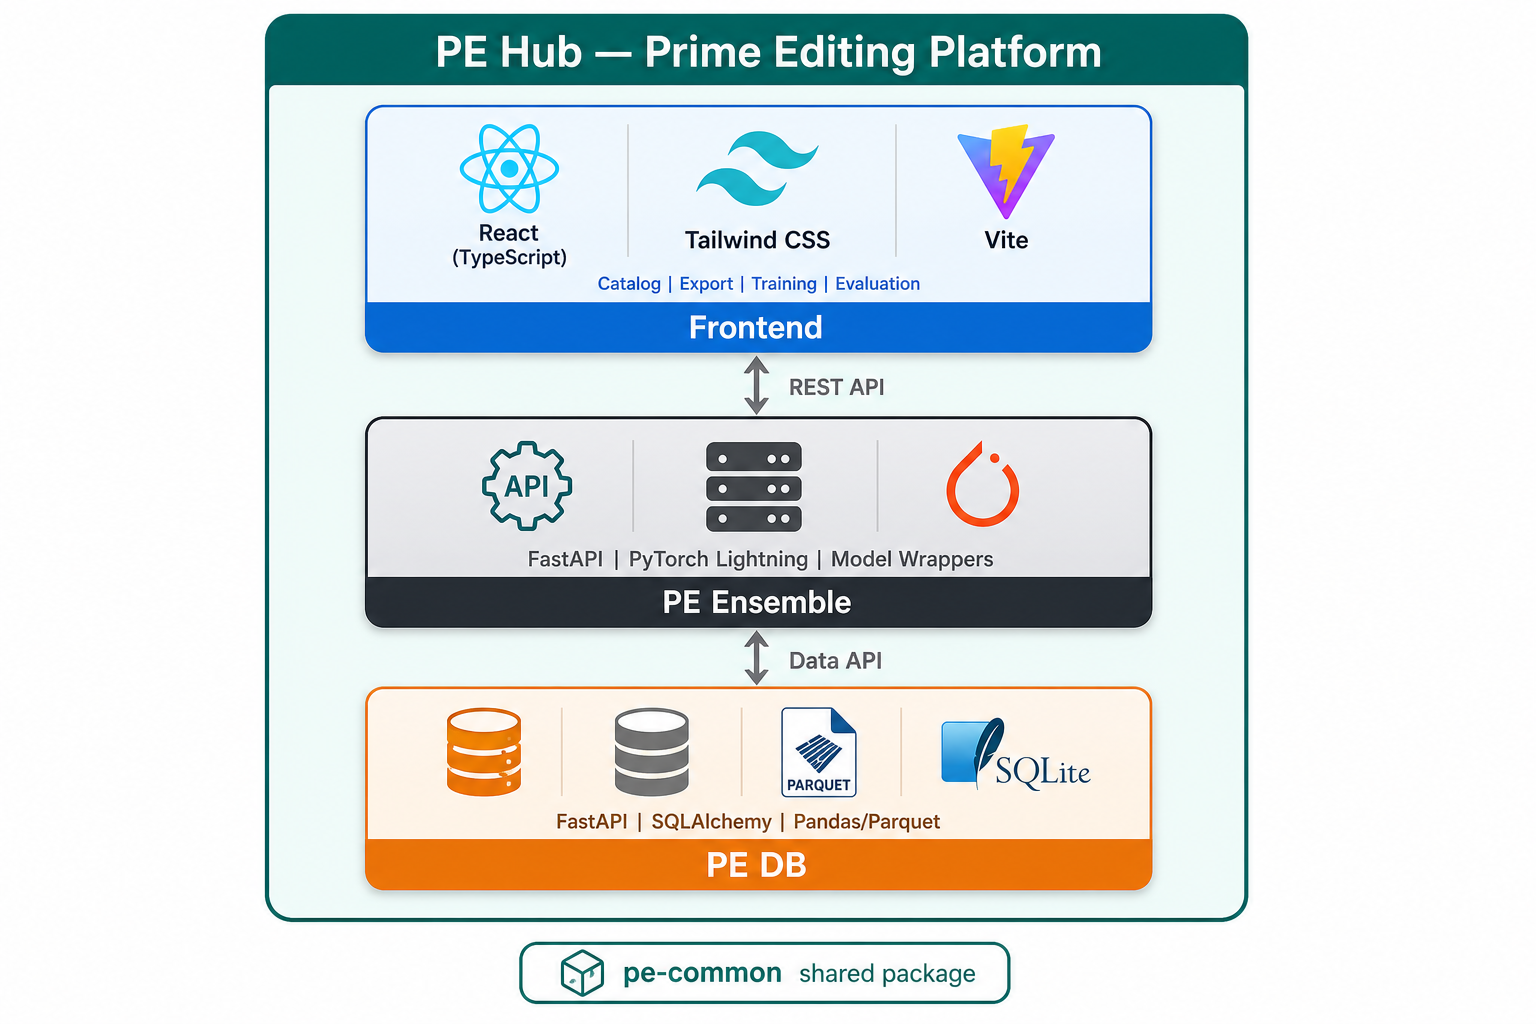
\includegraphics[width=0.8\linewidth]{diagrams/illustration/pe-platform-software-stack.png}
    \caption{Software Stack of PE Hub}
    \label{fig:pe-hub-architecture}
\end{figure}


\subsubsection{Using PE Hub}

In web deployment, PE Hub communicates with PE-DB and PE Ensemble through HTTP endpoints. PE Ensemble obtains model-formatted data from PE-DB, and long-running operations return a job identifier for status and log retrieval. The compute scheduler maintains a queue for each available device and runs one scheduled job at a time per device, supporting CPU, CUDA, and Apple MPS where the selected model permits. Requests, manifests, logs, and results are stored on the filesystem, allowing completed jobs and registered weights to be inspected after execution.

For cluster use, the \nolinkurl{pedb} and \nolinkurl{peen} command-line interfaces invoke the backend Python libraries directly. Batch jobs need the software environment and data files but no running web server. The repository supplies environment setup scripts, SLURM examples for Oxford ARC, and DVC configuration examples for synchronizing large datasets and results. Data filters, split assignments, weight identifiers, and training configuration are shared across the web, API, and command-line paths.

\subsubsection{Introducing Custom Models}

A recurring cost of publishing a new pegRNA-efficiency model is rebuilding the surrounding infrastructure: study tables must be parsed, sequences reconstructed, splits defined without locus leakage, and published checkpoints re-run under a protocol that is rarely identical to the original paper. PE Hub is intended to remove that work for model authors. The catalogued PE-core tables, named design rules, leakage-aware partitions, and vendor weight sets are already in place; an author supplies the architecture, not a second copy of the data and evaluation stack.

New models are registered as plugins rather than by editing PE Ensemble or PE-DB. A bundle contains a manifest, a wrapper that implements the common model interface, and, when the architecture needs its own input columns, a converter from PE-core; a starter template and an optional pretrained-weight directory are provided. The plugin manager checks the declared files and runs conversion and model-operation smoke tests before activation, so a broken wrapper cannot enter the Train or Benchmark menus. Activated wrappers join the PE Ensemble registry and their converters are registered in PE-DB; the web interface provides upload and validation controls. Once active, the new model uses the same data-selection, training, evaluation, ensemble, and design workflows as DeepPrime, OPED, and PRIDICT2, so a comparison against current methods is a shared experiment rather than a separately engineered pipeline. The authors can also submit pull requests to permanently add their model into PE-Hub as an additional vendor model after thourough testing.


\section{Result}

Using the CLI and Web Portal, a number of experiments were conducted to evaluate the performance of the models on the datasets. The results are presented in the following sections.

\subsection{Benchmarking Vendor Models}

\begin{figure}[ht]
    \centering
    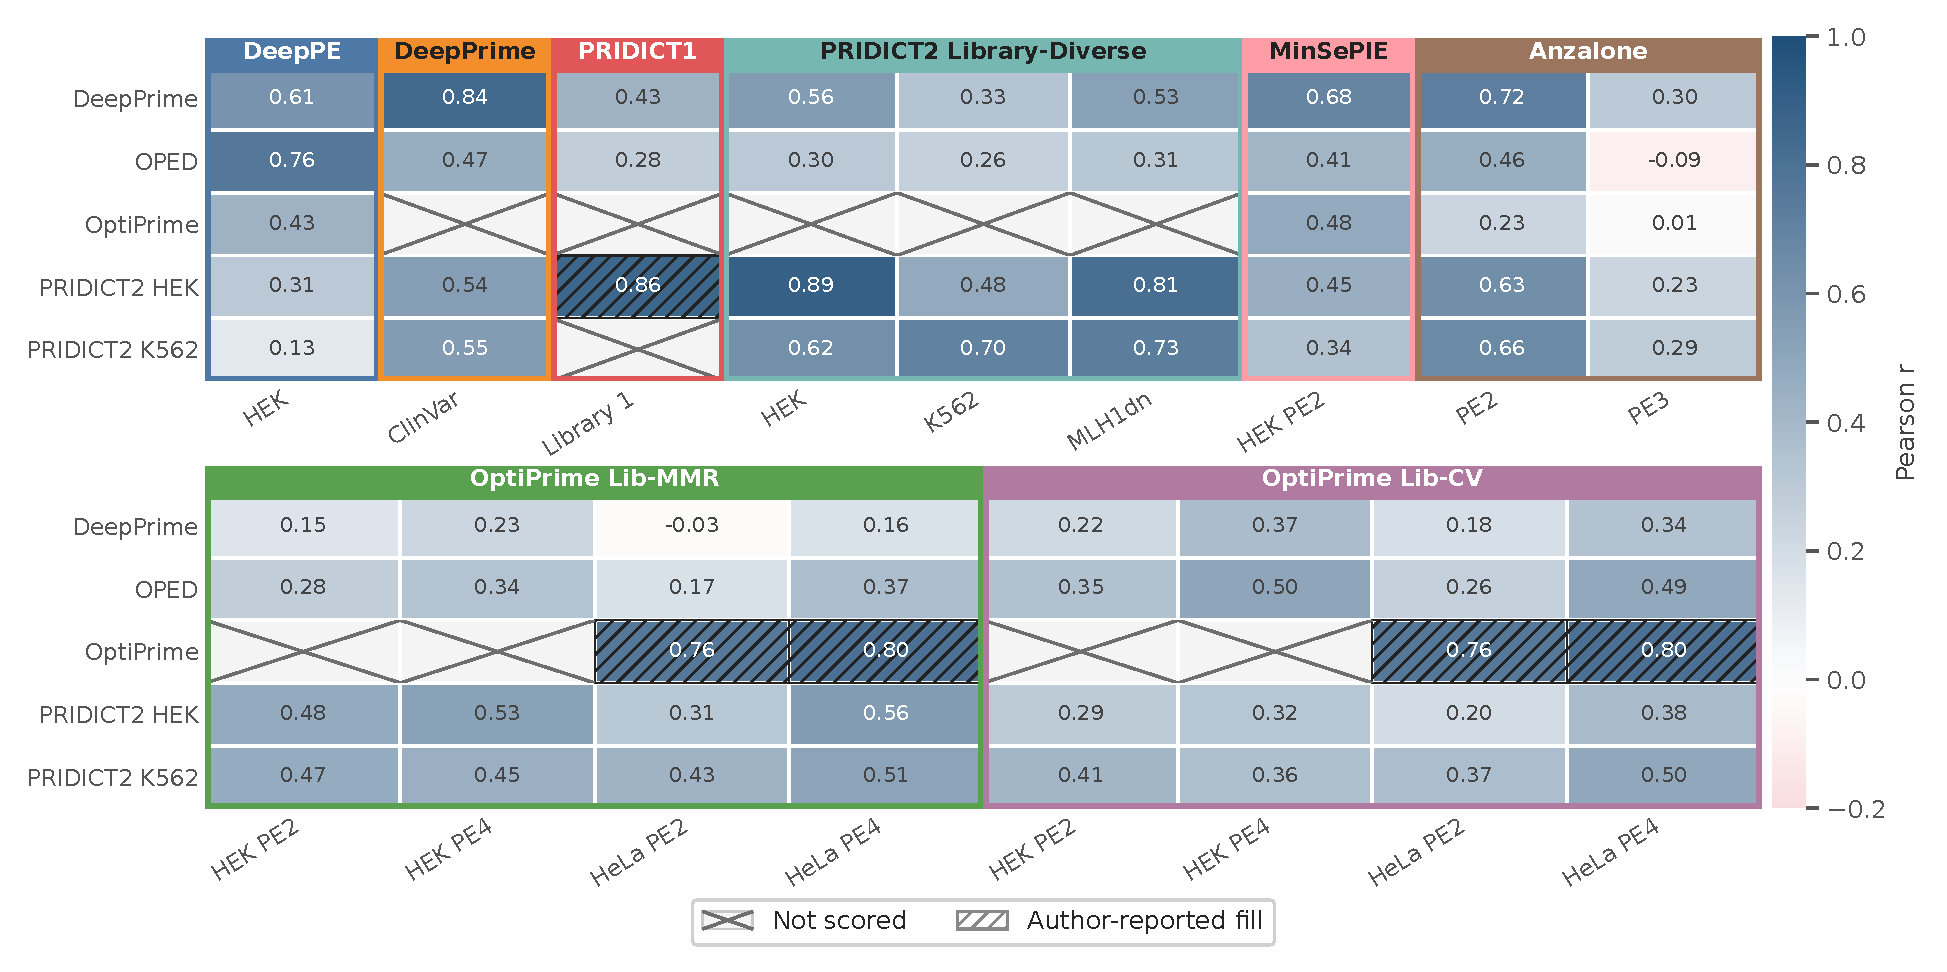
\includegraphics[width=\textwidth]{diagrams/eval_pearson_heatmap.pdf}
    \caption{Pearson $r$ between vendor-model predictions and measured intended-edit efficiency. Columns are study panels; rows are weight sets. The first row includes Anzalone 2019 HEK293T PE2 and PE3 (full Easy-Prime-reformatted sheet). Cells marked with an X and hatched cells cannot be measured in PE-Hub due to significant in-domain leakage. If author reported value can be found in their respective paper, it is filled into the heatmap in hatched cell. If no meaningful result can be found, the model is marked with X and is not scored.}
    \label{fig:pearson-heatmap}
\end{figure}

\begin{figure}[p]
    \centering
    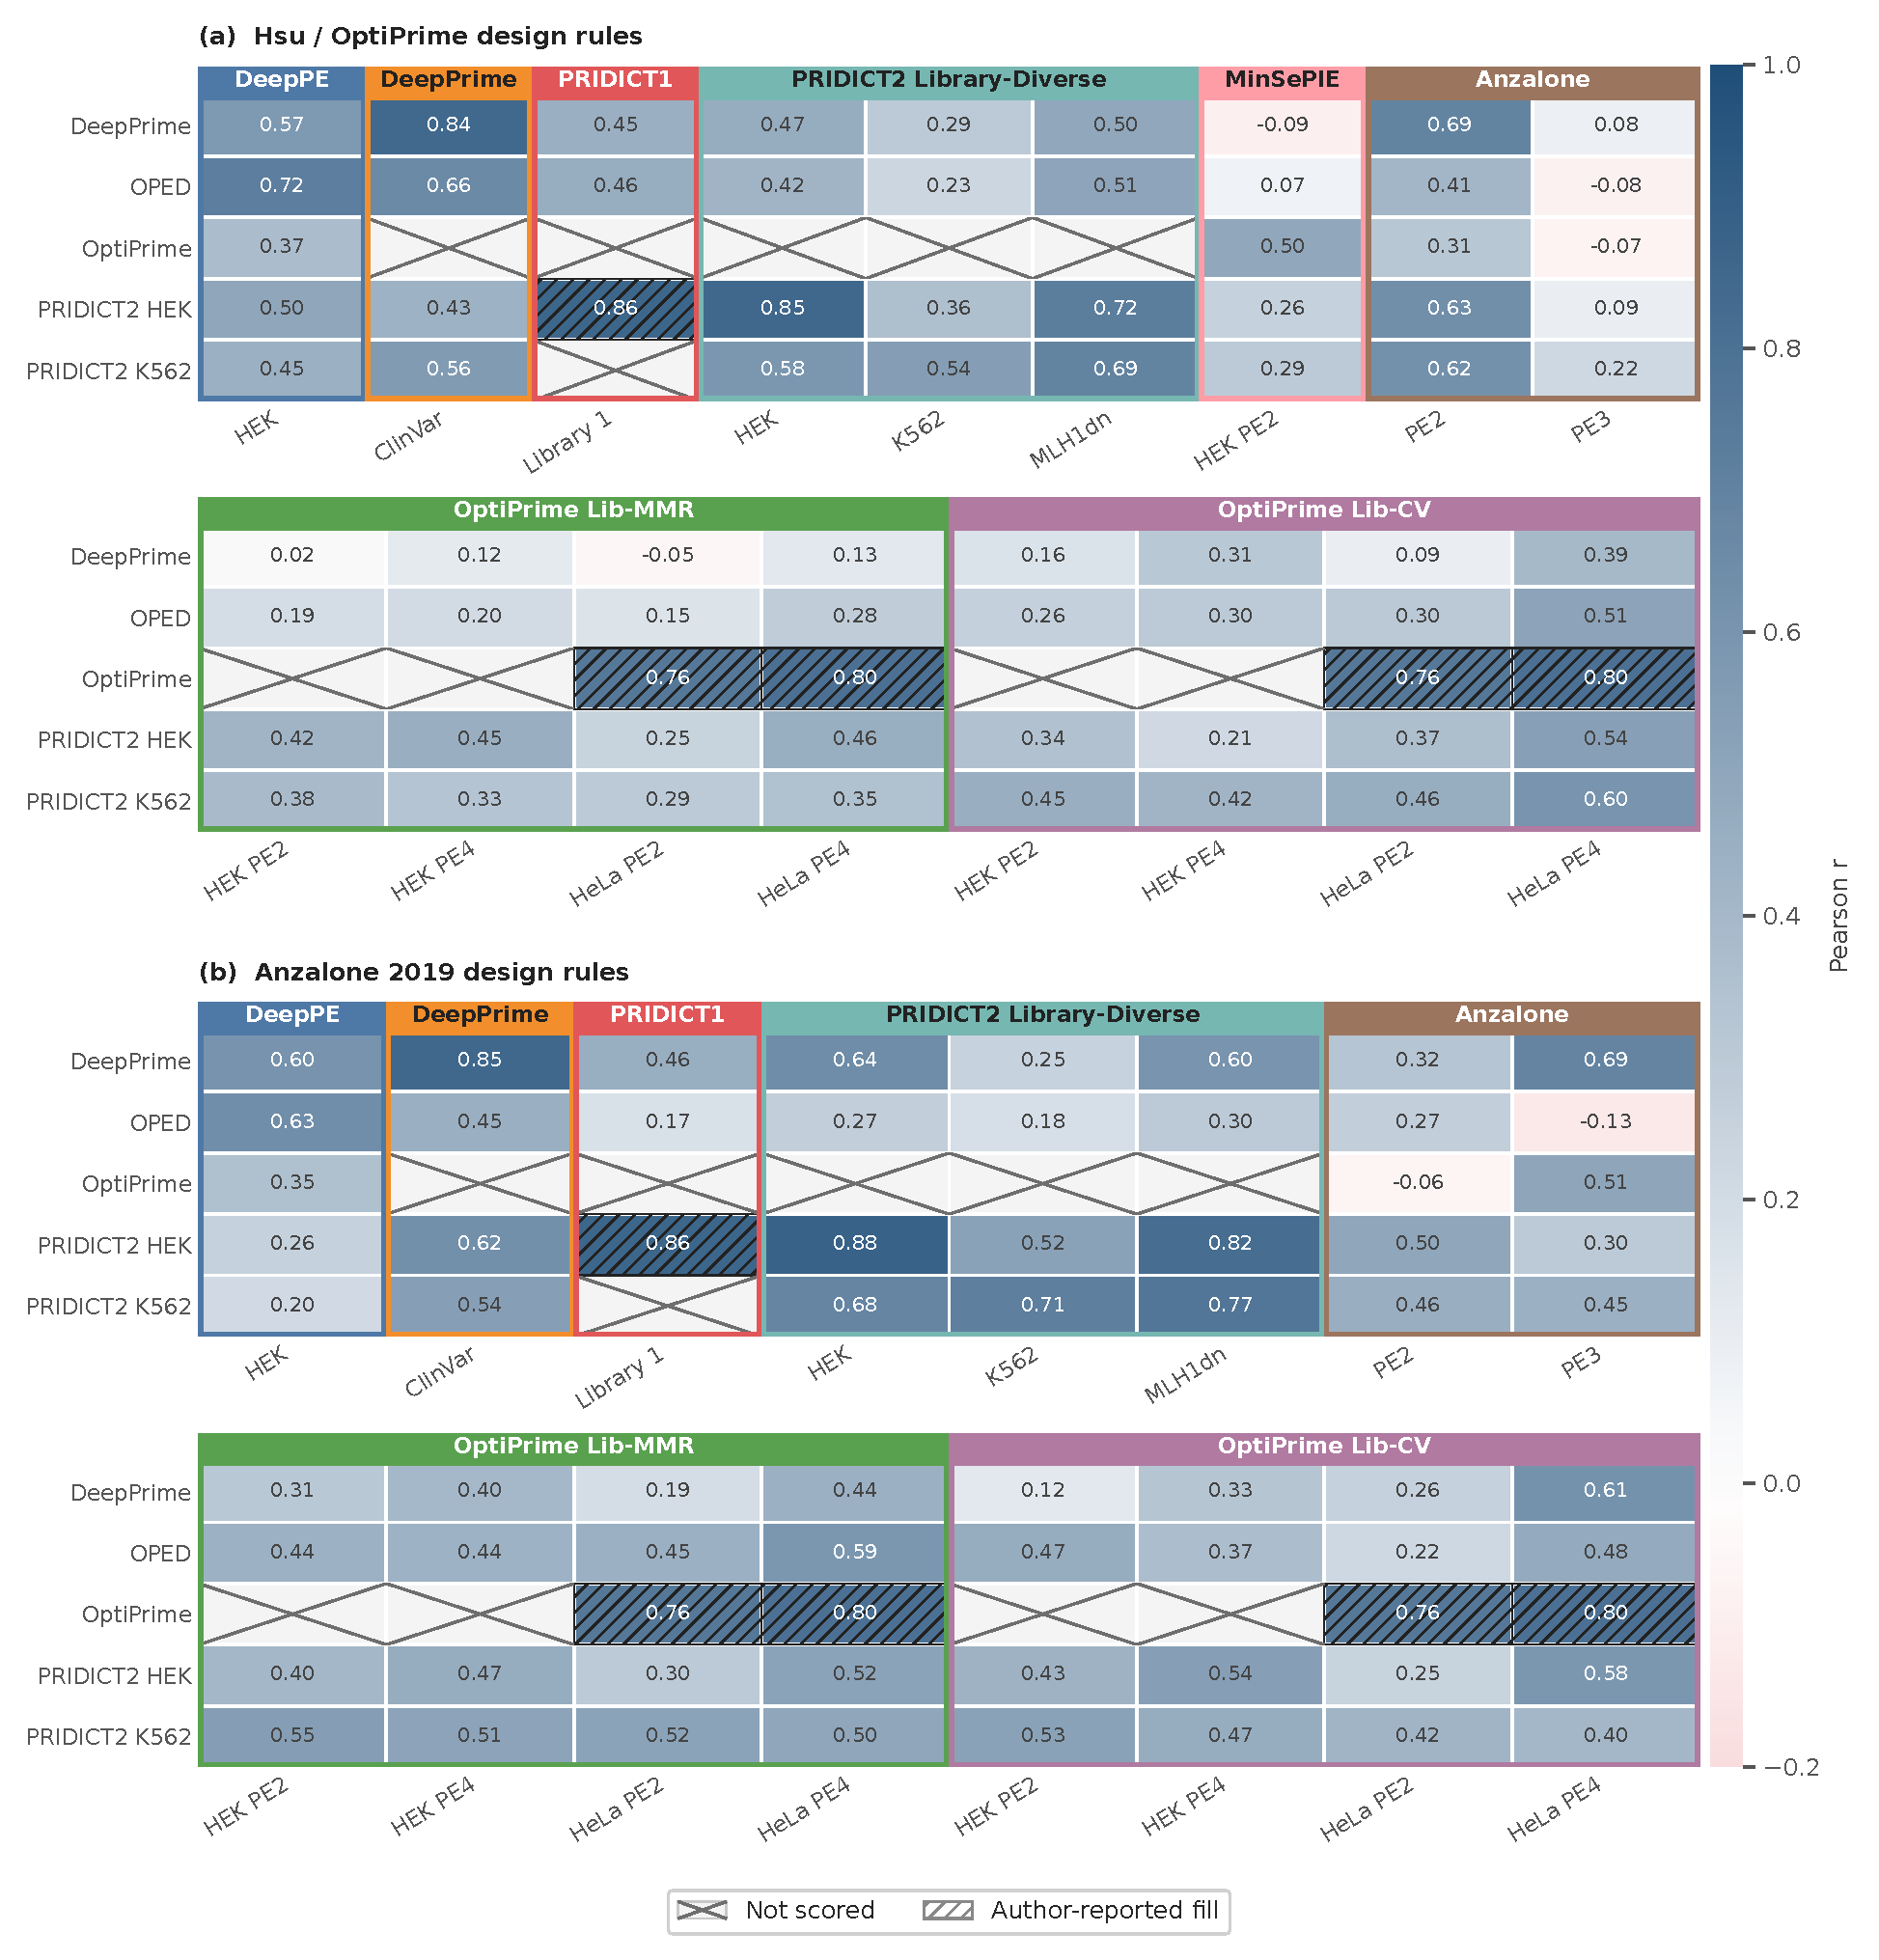
\includegraphics[width=\textwidth]{diagrams/eval_pearson_heatmap_design_rules.pdf}
    \caption{(a)~Hsu / OptiPrime filter used here: PBS length 13 and first RTT nucleotide not C.
    (b)~Anzalone 2019 starting recommendations (PBS 10--16\,nt, PBS GC 40--60\%, RTT 10--16\,nt, first RTT nucleotide not C); MinsePIE is omitted because no pegRNA has an RTT in that window.
    Pearson $r$ on the filtered subset of each sheet, including Anzalone PE2/PE3 on the first row and the OptiPrime model row; hatched cells remain author-reported fills.}
    \label{fig:pearson-heatmap-design-rules}
\end{figure}

As a starting point, the four vendor weight sets---DeepPrime~\cite{yuPredictionEfficienciesDiverse2023}, OPED~\cite{liuDesignPrimeeditingGuide2023}, OptiPrime~\cite{hsuMechanisticMachineLearning2026}, and the two PRIDICT2.0 heads~\cite{mathisMachineLearningPrediction2024}---were evaluated without retraining. Pearson $r$ between predicted and measured intended-edit efficiency is the heatmap metric (\autoref{fig:pearson-heatmap}). A very conservative leak prevention strategy was applied, overlapping training loci~(across multiple datasets for model using transfer learning) are excluded from the test set when a author provided test split is available. In-domain evaluation of a sheet that has no recoverable author test split is aborted rather than scored on a synthetic partition of the training loci.

\subsubsection{Participating datasheets}

The heatmap is restricted to screens that are large enough for a stable correlation: typically thousands of pegRNA--target pairs, or a locus-grouped holdout of that order. The exception is Anzalone et al.\ 2019, scored in full (no holdout) as the standard external PE2/PE3 HEK293T check. 

The datasets that remain are:

\begin{itemize}
    \item \textbf{DeepPE HEK293T} (\nolinkurl{deeppe-ht}, \nolinkurl{deeppe-type}, \nolinkurl{deeppe-position}, and HEK endogenous rows pooled). Kim et al.\cite{kimPredictingEfficiencyPrime2021} is the original high-throughput PE2 reporter screen and the training domain of OPED. Author-fold test rows give $n \approx 5{,}000$.
    \item \textbf{DeepPrime ClinVar} (\nolinkurl{deepprime-clinvar}). Yu et al.\cite{yuPredictionEfficienciesDiverse2023} measured ${\sim}$259{,}000 pegRNAs on synthetic 74~bp contexts in HEK293T; the author \texttt{Test} fold used here has $n \approx 28{,}000$. This is the training domain of \nolinkurl{DeepPrime\_base}.
    \item \textbf{PRIDICT Library 1} (\nolinkurl{library1}). Mathis et al.\cite{schwankgeraldPredictingPrimeEditing2023} screened 92{,}423 HEK293T reporter pegRNAs. No vendor hold-out is distributed, so in-domain scoring of PRIDICT2 and OptiPrime cannot be performed given our limited information.
    \item \textbf{PRIDICT2 Library-Diverse} in HEK293T, K562, and K562-MLH1dn (\nolinkurl{library-diverse}). Mathis et al.\cite{mathisMachineLearningPrediction2024} extended the reporter format to longer and more mixed edits; each cell-line sheet has $n \approx 4{,}000$--$4{,}500$ on the fold-matched test. This is the fine-tuning domain of the two PRIDICT2 heads.
    \item \textbf{MinsePIE HEK PE2} (pooled insertion screens at endogenous HEK3 / EMX1 / FANCF / CLYBL). Koeppel et al.\cite{koeppelPredictionPrimeEditing2023} is the only large insertion-centric set ($n = 4{,}301$), with a median insert length of 18~nt.
    \item \textbf{Anzalone 2019 HEK PE2 and PE3} (\nolinkurl{anzalone-endo}). Easy-Prime-reformatted endogenous designs, $n = 199$ (PE2) and $n = 278$ (PE3). Every remaining row is scored (no 20\% holdout). Yu et al.\ reported DeepPrime $r = 0.74$ on the PE2 set (Fig.~3H).
    \item \textbf{OptiPrime Lib-MMR and Lib-CV}, HEK293T and HeLa cell lines edited with PE2 and PE4. Hsu et al.\cite{hsuMechanisticMachineLearning2026} screened ${\sim}$10{,}000 pegRNAs per library in a lentiviral reporter. HEK293T is mismatch-repair deficient relative to HeLa; PE4 co-expresses dominant-negative MLH1. A 20\% locus-grouped holdout devised by PE Hub ($n \approx 1{,}500$--$2{,}100$) is scored for every model that is not in-domain.
\end{itemize}

These panels therefore cover the training domains of all four models, plus three transfer tests: long endogenous insertions (MinsePIE), the Anzalone 2019 arrayed endogenous set, and an MMR-stratified PE2/PE4 pair (Hsu).

\subsubsection{Missing scores and author-reported fills}

Blank cells are evaluations that PE-hub refuses to run. OptiPrime was trained on the union of Lib-MMR, Lib-CV, Library~1, ClinVar, and Library-Diverse, with protospacer-stratified cross-validation whose fold membership is not in the deposited tables~\cite{hsuMechanisticMachineLearning2026}. Scoring those sheets with a random holdout would test training loci, so ClinVar, Library~1, and Library-Diverse stay empty for OptiPrime. The PRIDICT2 K562 head is likewise blank on Library~1: that library is HEK293T-only, and there is no K562-head paper number to display.

Hatched cells are not PE-hub measurements. When an in-domain job aborts, the heatmap copies a published figure where one exists and marks it as an author-reported fill:

\begin{itemize}
    \item PRIDICT2 HEK $\times$ Library~1 uses the PRIDICT (not PRIDICT2) grouped five-fold CV from Mathis et al.\ 2023, $r = 0.86$ / $\rho = 0.85$\cite{schwankgeraldPredictingPrimeEditing2023}. PRIDICT2.0 was subsequently trained on every Library~1 locus, so this fill is a different model on a different protocol.
    \item OptiPrime $\times$ Lib-MMR / Lib-CV uses Hsu et al.\ Fig.~4 only for HeLa PE2 and HeLa PE4 ($r = 0.760$ / $0.803$), the published test-set scatters with Lib-MMR and Lib-CV pooled. HEK PE2 and HEK PE4 stay blank: Hsu quotes a four-condition mean ($r = 0.723$) but not HEK-only or per-library correlations, so filling those cells would overstate a condition-matched result\cite{hsuMechanisticMachineLearning2026}. The HeLa numbers are repeated across both library columns.
\end{itemize}

Where a close protocol match can be measured, PE-hub replicates the paper's result: DeepPrime on ClinVar $r = 0.834$ versus $0.84$\cite{yuPredictionEfficienciesDiverse2023}; PRIDICT2 HEK on Diverse HEK $r = 0.895$ versus $0.90$, and K562 on Diverse K562 $r = 0.700$ versus $0.70$\cite{mathisMachineLearningPrediction2024}; OPED on Anzalone PE2 $r = 0.46$ vs $r = 0.469$. Remaining gaps are therefore transfer, domain shift, or an intentional protocol difference, not a loading error.




\subsubsection{Evaluation Results}

\paragraph{DeepPE HEK293T.}
OPED is in-domain here and reaches $r = 0.76$ ($n = 5{,}060$), close to figure reported by Liu et al. ($r = 0.769$ on the HT-test alone, $n = 4{,}457$)\cite{liuDesignPrimeeditingGuide2023}. The shortfall is likely a protocol difference, since this evaluation pools HT, type, and position instead of HT-test alone. DeepPrime transfers reasonably ($r = 0.61$): ClinVar and DeepPE are both HEK reporter screens of short edits. OptiPrime ($r = 0.44$, leftover-excluded $n = 5{,}021$) and both PRIDICT2 heads ($r \approx 0.13$--$0.31$) are weaker, as expected for models whose training libraries post-date DeepPE and use different reporter geometries.

\paragraph{DeepPrime ClinVar.}
\nolinkurl{DeepPrime\_base} on the author test fold is the cleanest in-domain cell in the matrix: $r = 0.84$ ($n = 28{,}221$) against Yu's $0.84$ ($n = 28{,}883$)\cite{yuPredictionEfficienciesDiverse2023}. The small $n$ drop is leftover-exclusion of protospacers that appear in both the published train and test tables under our leak prevention (\nolinkurl{DeepPrime\_base} records train-fold loci only), compared with the author's split on the entire pegRNA sequence. OPED ($r = 0.47$) and PRIDICT2 ($r \approx 0.54$--$0.55$) see the same sheet as transfer. OptiPrime is blank on the heatmap (Hsu trained on ClinVar without Yu's holdout).

\paragraph{PRIDICT Library 1.}
No author test split is on the sheet, so PRIDICT2 and OptiPrime cannot be measured in-domain on the heatmap. The hatched $0.86$ is the earlier PRIDICT CV number discussed above. The measured column is transfer of DeepPE-trained OPED ($r = 0.28$) and ClinVar-trained DeepPrime ($r = 0.43$). Liu et al.\ reported $r = 0.912$ only after \emph{retraining} OPED on the Library~1 split\cite{liuDesignPrimeeditingGuide2023}; that experiment is not this heatmap row.

\paragraph{PRIDICT2 Library-Diverse.}
Fold-matched evaluation of each PRIDICT2 head on its own cell line reproduces Mathis et al.: HEK$\to$HEK $r = 0.90$, K562$\to$K562 $r = 0.70$\cite{mathisMachineLearningPrediction2024}. The evaluation data points dropped due to the stricter leak prevention strategy did not affect the correlation. Cross-cell behaviour is the more informative result. HEK293T is mismatch-repair deficient; K562 is proficient; K562-MLH1dn phenocopies deficiency with dominant-negative MLH1, as PE4 does in the Hsu screens. The HEK head's performance collapses on MMR-proficient K562 ($r = 0.48$) and recovers on MLH1dn ($r = 0.81$, $\rho = 0.88$, matching the paper). The K562 head is more consistent ($r = 0.62$ / $0.70$ / $0.72$; Spearman already ${\sim}0.81$--$0.83$ in Mathis). That pattern is in the published numbers and in the efficiency distributions of the three sheets (median intended-edit ${\sim}11\%$ / $0.8\%$ / $3.8\%$). It is not a swapped-head bug: the K562 decoder was never an MMR classifier, and MLH1dn was an evaluation condition, not a third training head.

DeepPrime's Spearman on these sheets ($R = 0.79$ / $0.59$ / $0.75$) is in the same range as Yu's $\leq 3$~bp subset of Library-Diverse; Pearson is lower because the unfiltered library includes edits outside DeepPrime's 1--3~bp training support. OptiPrime is again blank on the heatmap (Hsu trained on this library). OPED remains a modest transfer model ($r \approx 0.26$--$0.31$).

\paragraph{MinsePIE HEK PE2.}
This column is almost entirely insertions (median 18~nt, RT templates often $>50$~nt) at a handful of endogenous loci, still in HEK293T PE2. DeepPrime reaches $r = 0.68$ on the leftover-excluded subset ($n = 13{,}826$). OPED retains a usable ranking on the smaller PE-Hub holdout ($r = 0.41$, $n = 4{,}301$), consistent with its nucleotide decoder not being hard-capped at 3~bp. OptiPrime on the same holdout still ranks inserts ($\rho = 0.52$) relatively well but Pearson falls to $r = 0.10$, showing that predicted efficiencies no longer scale linearly with the long-insert measurements. The PRIDICT2 surprise is that the HEK head ($r = 0.45$) only modestly beats the K562 head ($r = 0.34$) on a HEK MMR-deficient sheet. If head--MMR matching were the dominant effect, HEK should win by more. The more plausible reading is edit class: PRIDICT2's library-diverse insertions stop at 15~nt (median 7), whereas MinsePIE is a long-insert, few-locus endogenous assay. The heatmap cell is not an RC or HAP1 mix-up; those panels were excluded.

\paragraph{Anzalone 2019 HEK PE2 and PE3.}
This is the small arrayed endogenous set, scored in full rather than on a 20\% holdout. PE3 leftover-excludes loci that overlap vendor training spacers ($n = 213$ of $278$ for DeepPrime, OptiPrime, and PRIDICT2; OPED keeps all $278$). DeepPrime reaches $r = 0.72$ / $\rho = 0.69$ on PE2 against Yu et al.\ $r = R = 0.74$ (Fig.~3H)\cite{yuPredictionEfficienciesDiverse2023}. PRIDICT2 HEK ($r = 0.63$, $\rho = 0.69$) matches Mathis et al.\ 2024 on Anzalone ($r = 0.63$, $R = 0.69$, $n = 181$). The K562 head is similar in Pearson ($r = 0.66$). After restoring Hsu's target geometry, OptiPrime reaches $r = 0.64$ ($\rho = 0.68$, $n = 199$) on PE2; OPED's $r = 0.46$ matches Liu's reported value. PE3 remains a different editor: leftover-excluded OptiPrime is $r = 0.09$ ($n = 212$), and every model falls to $r \approx 0.00$--$0.30$.

\paragraph{OptiPrime Lib-MMR.}
Lib-MMR was built as an MMR assay: diverse substitutions and indels at 200 exonic sites, HEK293T versus HeLa, PE2 versus PE4\cite{hsuMechanisticMachineLearning2026}. OptiPrime's HeLa cells are hatched author fills; HEK stays blank. Among measured models, PRIDICT2 HEK behaves as the Diverse HEK head would predict. It is strongest on HEK PE2/PE4 ($r = 0.48$ / $0.53$) and on HeLa PE4 ($r = 0.56$), and weakest on MMR-proficient HeLa PE2 ($r = 0.31$). The K562 head drops less on that cell ($r = 0.43$), again matching a decoder trained in an MMR-proficient line. OPED follows the same PE2/PE4 direction at lower absolute $r$ ($0.17$ on HeLa PE2, $0.37$ on HeLa PE4).

DeepPrime on HeLa PE2 is the clear outlier ($r = -0.03$, $\rho = 0.03$), likely a result of missing essential data. Hsu's designed targets start at the spacer, so every Lib-MMR WT74 is left-padded with \texttt{NNNN}; DeepPrime encodes \texttt{N} as a zero channel, wiping the 4~bp of genomic context the CNN was trained on. Lib-CV, which supplies real 4~bp flanks, is higher for DeepPrime in every matched cell. 

\paragraph{OptiPrime Lib-CV.}
Lib-CV is a ClinVar-correction library (${\sim}$91\% substitutions, including silent-edit combinations meant to evade MMR)\cite{hsuMechanisticMachineLearning2026}. PE4 still lifts every model relative to PE2, but the HEK-head collapse from HEK PE2 to HeLa PE2 is almost absent ($r = 0.29 \to 0.20$), unlike Lib-MMR ($0.48 \to 0.31$). This is expected as Lib-MMR is enriched with MMR-evasive designs, such as silent edits alongside targeted modification\cite{hsuMechanisticMachineLearning2026}.

DeepPrime is higher than on Lib-MMR throughout, including HeLa PE2 ($r = 0.18$), consistent with real WT74 sequence rather than \texttt{NNNN} pads; Spearman ($R = 0.33$) shows that a rank signal remains after Pearson is compressed by low PE2 efficiencies. OPED is the strongest measured transfer model on this library ($r = 0.26$--$0.50$), still well below the hatched OptiPrime HeLa fills.

\subsubsection{Design-rule filtered evaluation}

Hsu et al.\ argued that many published pegRNAs would never be ordered in practice, and that correlations for other models may therefore look better than they should~\cite{hsuMechanisticMachineLearning2026}. We repeated the unfiltered matrix of \autoref{fig:pearson-heatmap} under the two named PE-DB rulesets (Methods): Hsu's PBS and RTT-start constraints (\nolinkurl{optiprime}) and the Anzalone et al.\ 2019 starting recommendations (\nolinkurl{anzalone})~\cite{anzaloneSearchandreplaceGenomeEditing2019}. Layout and colour scale are unchanged; but cell lines ended up with no data after filtering were dropped (\autoref{fig:pearson-heatmap-design-rules}).

The \nolinkurl{optiprime} preset is a subset of Hsu's Methods.
Hsu's Methods also prescribe 3$'$ homology of $9+L$ (substitutions) or $19+L$ (insertions and deletions), then a length nudge so the RTT does not start with C. We leave that clause out of the named \nolinkurl{optiprime} preset. It fits single-base Lib-MMR substitutions exactly, but the deposited sheets do not follow it more generally: Lib-MMR multi-base edits and short indels sit on ${\sim}$15\,nt arms and longer indels on ${\sim}$20\,nt arms rather than $19+L$, while Lib-CV silent-edit combinations keep ${\sim}$10\,nt arms rather than $9+$ (substitution span). Enforcing the formula would discard a large share of Hsu's own holdouts for reasons other than a bad PBS or a leading C, so only the two checks are applied.

Under that PBS/RTT filter, Hsu's Lib-MMR / Lib-CV panels are essentially intact (${\sim}$95--100\% of the original count). External sheets are more affected: DeepPE HEK leftover-excluded $n$ for DeepPrime drops ($1{,}033 \to 155$), ClinVar's leftover-excluded author test shrinks further ($28{,}221 \to 1{,}343$), and Library~1 / Library-Diverse keep about one-sixth of their unfiltered holdouts. Anzalone PE2 keeps $n = 68$ of $199$ (DeepPrime $0.72 \to 0.69$; PRIDICT2 HEK $0.63 \to 0.63$; OptiPrime $0.64 \to 0.59$); PE3 ($n = 100$) collapses toward zero for every model, thus the rank changes are not meaningful. Pearson values on the large libraries still move little in a consistent direction. DeepPrime is slightly down on DeepPE ($0.61 \to 0.57$), almost unchanged on ClinVar and Library~1, and slightly down on Library-Diverse HEK ($0.56 \to 0.47$). OPED falls modestly on DeepPE ($0.76 \to 0.72$) and collapses on the remaining MinsePIE inserts ($0.41 \to 0.07$), while rising on Library~1 ($0.28 \to 0.46$). PRIDICT2's in-domain Diverse HEK cell softens slightly ($0.90 \to 0.85$), and transfer onto Hsu's libraries shifts by only a few hundredths.

Anzalone's 10--16\,nt RTT window produces stronger filtering (\autoref{fig:pearson-heatmap-design-rules}b). It empties MinsePIE (median insert 18\,nt), and keeps only 3--8\% of Lib-MMR / Lib-CV, leaving $n \approx 50$--$160$---too small to read ranking changes. The Anzalone PE2 column itself shrinks to $n = 26$, which again are too small to interpret. Anzalone PE3 keeps $n = 43$--$44$, resulting in big improvements for all models other than OPED. On the larger external remainders the picture is again mixed: DeepPE OPED falls ($0.76 \to 0.63$), ClinVar PRIDICT2 HEK rises ($0.54 \to 0.62$), and DeepPrime on Library-Diverse HEK improves ($0.56 \to 0.64$). 

In line with other models, OptiPrime was not consistently helped by either filter, with a correlation drop on both DeepPE and Anzalone PE2. Its performance on MinsePIE inserts did improve in terms of linear correlation, but Spearman rank suffered a slight drop ($r = 0.10 \to 0.29$, $\rho = 0.52 \to 0.49$, $n = 13{,}826$).

So Hsu is right that many published designs fail simple practitioner checks on PBS and RTT start base, and the $n$ drop on external libraries shows that. What the filtered matrices do not support is the stronger claim that other models look good mainly because of those designs: removing them helps some cells and hurts others, including OptiPrime. 

\subsection{From-scratch base-weight training}

The vendor matrix above scores published checkpoints. To ask how the three deep architectures compare when each is trained from random initialization on the same sheet and the same holdout protocol, a second matrix was run on Oxford ARC: DeepPrime, OPED, and PRIDICT2, each trained without loading vendor weights (\nolinkurl{load\_pretrained=false}). OptiPrime is omitted due to its training integration limitation stated in section \ref{subsubsection:models}.

\paragraph{Protocol.}
Every cell uses the datasheet-benchmark runner under a fixed \nolinkurl{holdout\_3} split (70/15/15 train/validation/test by locus group, base seed 42). For each of three split seeds (42, 43, 44) the job runs ten Optuna trials that maximize validation Spearman, registers weights from the best trial, and evaluates on that seed's held-out test partition in the same SLURM allocation. Epoch budgets are not searched: early stopping (patience 10) is the primary stop, with a large \nolinkurl{max\_epochs} backstop. Unlike the vendor evaluation, author folds are not used, so Library~1 (which has no deposited PRIDICT holdout) and ClinVar / DeepPE can be compared under the same random split across seeds.

Six studies and 15 datasheets were used during the training: PRIDICT Library~1 (HEK293T PE2), Library-Diverse as three separate sheets (HEK, K562, K562-MLH1dn), DeepPrime ClinVar (HEK293T PE2), DeepPE HEK pooled HT/type/position/endo, MinsePIE HEK PE2 insertion screens, and OptiPrime Lib-MMR / Lib-CV as eight sheets (HEK293T/HeLa $\times$ PE2/PE4). $15$ datasheets $\times$ $3$ models $\times$ $3$ seeds $= 135$ train--eval repeats. Jobs ran on ARC HTC L40S GPUs (typically short / 12\,h per seed; ClinVar OPED required resume of the Optuna study after timeouts).

\begin{figure}[p]
    \centering
    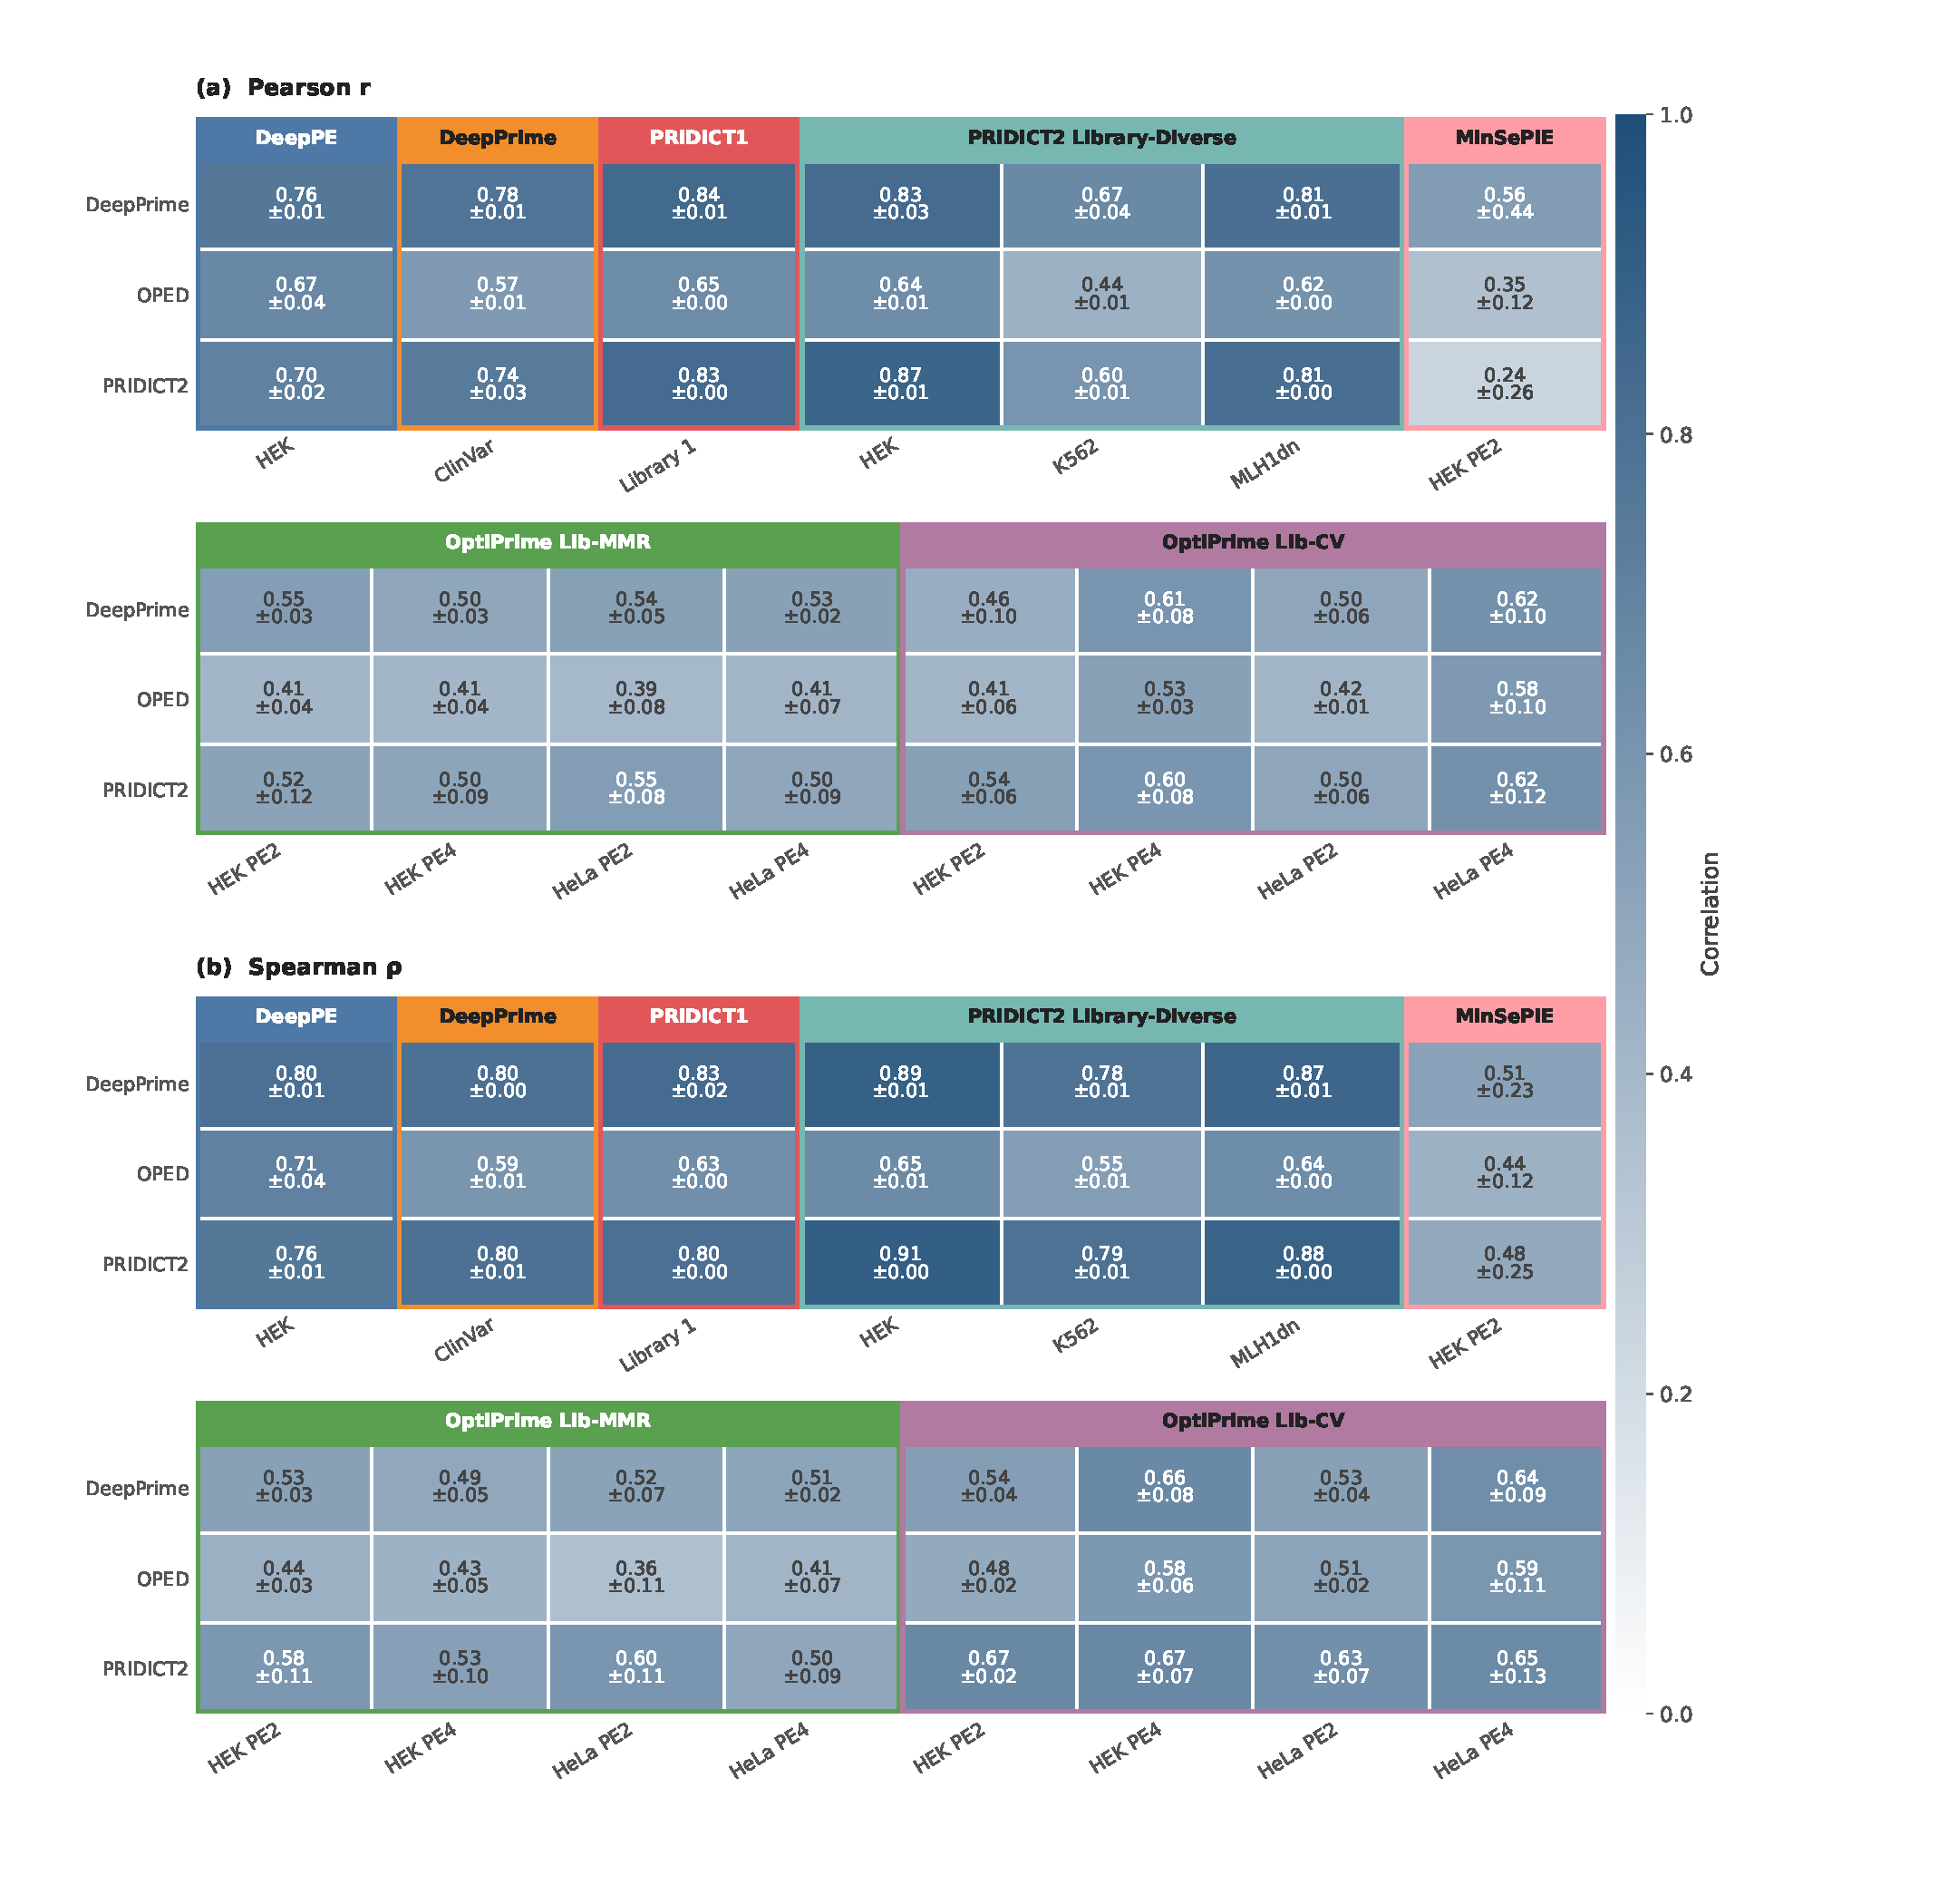
\includegraphics[width=\textwidth]{diagrams/scratch_correlation_heatmap.pdf}
    \caption{(a)~Pearson $r$ (mean $\pm$ s.d.\ over three holdout$_3$ seeds) for DeepPrime, OPED, and PRIDICT2.
    (b)~Spearman $\rho$ on the same matrix; rank correlations remain high on Library-Diverse K562 even where Pearson falls, consistent with a compressed efficiency scale on that MMR-proficient line.
    Library-Diverse is split by HEK / K562 / K562-MLH1dn, and Lib-MMR / Lib-CV by HEK293T/HeLa $\times$ PE2/PE4, matching \autoref{fig:pearson-heatmap}; Library~1, ClinVar, DeepPE, and MinsePIE are single-condition. Unlike that vendor matrix, every cell is an in-sheet train--test under the same protocol; no vendor weights or author-fold fills are used.}
    \label{fig:scratch-heatmaps}
\end{figure}

\paragraph{Results.}
\autoref{fig:scratch-heatmaps} summarizes test Pearson and Spearman.

On PRIDICT Library~1, DeepPrime and PRIDICT2 are essentially tied (Pearson $r = 0.84 \pm 0.01$ and $0.83 \pm 0.00$; Spearman $\rho \approx 0.83$ / $0.80$), while OPED lags ($r = 0.67$, $\rho = 0.65$). That ordering is the opposite of Liu et al.'s claim that OPED reaches $r = 0.91$ after retraining on Library~1~\cite{liuDesignPrimeeditingGuide2023}: under a shared holdout and a common Optuna budget, OPED does not dominate this sheet.

DeepPrime ClinVar remains DeepPrime's strongest large-domain cell ($r = 0.78 \pm 0.01$, $\rho = 0.80$), close to the vendor ClinVar in-domain Pearson of $0.83$ in \autoref{fig:pearson-heatmap} despite the protocol change (author fold versus random holdout; leftover-exclusion off). PRIDICT2 is competitive ($r = 0.74$, $\rho = 0.80$); OPED trails ($r = 0.60$, $\rho = 0.61$). On DeepPE HEK, DeepPrime again leads ($r = 0.76$, $\rho = 0.80$), with PRIDICT2 and OPED essentially tied ($0.70$ / $0.76$ and $0.70$ / $0.73$)---so the architecture that was trained on DeepPE by Liu et al.\ is not the best from-scratch fit under this budget.

MinsePIE HEK PE2 is the unstable column. Mean Pearson looks moderate for DeepPrime ($0.56$) and weaker for OPED and PRIDICT2 ($0.26$ / $0.24$), yet seed-to-seed scatter is large (DeepPrime Pearson s.d.\ $0.44$; OPED $0.20$; PRIDICT2 $0.26$). The pooled insertion screens concentrate on a handful of endogenous loci, so a 15\% group holdout can change composition dramatically across seeds; the means alone are not reliable rankings.

On Library-Diverse, HEK and K562-MLH1dn remain high for DeepPrime ($r = 0.83$ / $0.81$) and PRIDICT2 ($r = 0.87$ / $0.81$), while K562 is lower in Pearson ($r = 0.67$ / $0.60$) with Spearman still high ($\rho = 0.78$ / $0.79$). That follows the compressed K562 efficiency scale (median intended-edit ${\sim}0.8\%$ versus ${\sim}11\%$ on HEK): the models rank pegRNAs after training on K562, but Pearson is harder on a low-efficiency assay. OPED follows the same HEK $\approx$ MLH1dn $>$ K562 order at lower absolute $r$ ($0.66$ / $0.63$ / $0.47$).

Performance on Lib-MMR is relatively flat across HEK/HeLa $\times$ PE2/PE4 for DeepPrime and PRIDICT2 ($r \approx 0.50$--$0.55$), whereas OPED spans a wider range ($r \approx 0.26$--$0.46$) with a PE2$\to$PE4 lift (HEK $0.26 \to 0.46$; HeLa $0.35 \to 0.44$). Lib-CV is higher and shows a PE4 lift for all three models (DeepPrime HEK $0.46 \to 0.61$, HeLa $0.50 \to 0.62$; PRIDICT2 $0.54 \to 0.60$ / $0.50 \to 0.62$; OPED $0.43 \to 0.54$ / $0.40 \to 0.58$), which is surprising given that the models were not designed to handle predicting substitutions accompanied by silent edits. Still, absolute Pearson on both Hsu panels remains well below the large HEK reporter sheets.

Overall, when vendor provenance and author folds are removed, DeepPrime and PRIDICT2 remain the stronger learners on the large HEK reporter sheets (Library~1, ClinVar, DeepPE, and Library-Diverse HEK / MLH1dn). OPED is consistently weaker under the same ten-trial budget. In-sheet training does not lift K562 Pearson to the HEK range, because that assay's efficiencies are much lower, nor does it raise Hsu's libraries to HEK-reporter levels, and MinsePIE remains noisy. 

\subsection{End-to-end PRIDICT2.0 reproduction}

\begin{table}[ht]
    \centering
    \small
    \begin{tabular}{@{}llcccc@{}}
        \hline
        Cell line & Source & Pearson $r$ & Spearman $\rho$ & $n$ / fold \\
        \hline
        HEK293T & Mathis et al.\ Fig.~1o & $0.90$ & $0.91$ & --- \\
        HEK293T & PE Hub reproduction (mean $\pm$ s.d.) & $0.896 \pm 0.007$ & $0.916 \pm 0.002$ & ${\sim}4{,}520$ \\
        K562 & Mathis et al.\ Fig.~1p & $0.70$ & $0.81$ & --- \\
        K562 & PE Hub reproduction (mean $\pm$ s.d.) & $0.620 \pm 0.008$ & $0.795 \pm 0.004$ & ${\sim}4{,}530$ \\
        \hline
    \end{tabular}
    \caption{PRIDICT2.0 Library-Diverse ensemble: published figures versus PE Hub end-to-end reproduction (five author folds; mean of Model~A and Model~B per fold).}
    \label{tab:pridict2-repro}
\end{table}

To showcase PE-DB's flexible data exportation and  PE-Ensemble's complete \emph{base training + transfer + ensemble} pipeline, I reproduced Mathis et al.'s PRIDICT2.0 construction on Oxford ARC using the reproduction scripts under \nolinkurl{scripts/experiments/pridict2-reproduction/}\cite{mathisMachineLearningPrediction2024}. The experiment was only performed once with the following protocol to avoid me biasing the result towards the original paper's numbers.

\paragraph{Protocol.}
Two bases were trained from scratch: Model~A on PRIDICT Library~1 alone, and Model~B on Library~1 merged with DeepPrime ClinVar. PRIDICT Library~1 used PE-DB defined holdout 3 70/15/15 split by locus group, and DeepPrime ClinVar used the author test fold $-1$ as test fold. Each base weight was then fine-tuned separately on Library-Diverse HEK and K562 for each author fold $x \in \{0,\ldots,4\}$, holding fold~$x$ out as test and splitting the remainder 70/15 for train/validation. During fine-tuning, encoder was frozen, decoder was trainable, single edit-efficiency head was used with \nolinkurl{MSEloss}. \nolinkurl{num\_epochs} was set to 100 as backstop, with early-stopping patience~10. That yields ten Model~A and ten Model~B checkpoints. The matching A/B pair was then mean-ensembled and scored the held-out author fold ($n \approx 4{,}520$ per fold).

\paragraph{Results.}
\autoref{tab:pridict2-repro} summarises fivefold mean $\pm$ s.d.\ on Library-Diverse against Mathis et al.\ Fig.~1o--p. On HEK the reproduction matches the paper within a few hundredths (Pearson $r = 0.896 \pm 0.007$ versus $0.90$; Spearman $\rho = 0.916 \pm 0.002$ versus $0.91$). On K562 Spearman is close to published range ($\rho = 0.795 \pm 0.004$ versus $0.81$) while Pearson is lower ($r = 0.620 \pm 0.008$ versus $0.70$). A likely cause is data composition: absolute efficiencies on K562 are much smaller than on HEK (median intended-edit ${\sim}0.8\%$ versus ${\sim}11\%$ for K562 vs HEK), so Pearson is more sensitive to calibration and to the MSE-only head used here. Fold-to-fold scatter is small on both heads (Pearson s.d.\ $<0.01$), indicating a stable pipeline rather than a single lucky fold.


% The point of the experiment is not to claim a new state of the art, but to show that PE-DB merge/export, PE Ensemble train/tune/evaluate/ensemble, registered weights, and fold-matched splits can re-run a non-trivial published recipe---base pretraining, transfer fine-tuning, and mean ensembling---under one toolchain, and land near the numbers that justified PRIDICT2.0 in the first place. Residual gaps (especially K562 Pearson) are consistent with deliberate protocol differences already noted for Library~1 (random holdout versus full-sheet pretraining) and with a single-efficiency MSE objective rather than the authors' full multi-outcome training stack.

\section{Discussion}

The main contribution of this work is a framework for comparing published prime-editing predictors under consistent, reproducible conditions. PE Hub combines a shared data schema, leak-proof data partitioning, model training and evaluation, as well as checkpoint registration to support comparisons across models and datasets. Where the original evaluation protocol can be reconstructed, PE Hub recovers the reported Pearson correlations. For example, DeepPrime on the ClinVar test fold, both PRIDICT2 heads on Library-Diverse HEK293T and K562, and OPED on Anzalone PE2. Additionally, reproducing PRIDICT2.0 from base pretraining through transfer fine-tuning and mean ensembling yielded close agreement with Mathis et al.\ on HEK293T ($r = 0.896$ versus $0.90$; $\rho = 0.916$ versus $0.91$). Together, these results demonstrate that PE-DB and PE Ensemble training and evaluation workflow has preserved the core capability of the models during integration and can reproduce a published pipeline end to end.

Using this framework, I investigated the transfer capability of vendor models with distinct architectures across a large variety of experimental settings. The result showed that regardless of the design of models and their training protocols, they still rely heavily on in-domain examples. The PRIDICT2 HEK head performed poorly in MMR-proficient K562 cells but recovered when MLH1dn induced an MMR-deficient state. A similar PE2–PE4 pattern was observed in Hsu’s HeLa screens. DeepPrime remained competitive on short HEK reporter edits and retained a rank correlation on long MinsePIE insertions, although Pearson correlation declined beyond the 1--3~bp edits represented in its training data. Input representation also affected performance: DeepPrime’s near-zero correlation on HeLa PE2 in Lib-MMR was associated with the \texttt{NNNN}-padded WT74 representation, whereas Lib-CV, which provides the actual 4~bp flanking sequences, yielded higher scores in every matched comparison. 
%  Transfer to PE3 was limited across all models, with Pearson correlations of approximately $0$--$0.30$ on Anzalone PE3. Published performance estimates should therefore be interpreted within their experimental domains, rather than assumed to extend to different MMR states, edit lengths, or nicking-guide protocols.
On the PE3 data produced through a more complex editing procedure, none of the vendor models successfully transferred, with Pearson correlations of approximately $0$--$0.30$ on Anzalone PE3 dataset. Published performance estimates should therefore be interpreted within their experimental domains, rather than assumed to extend to different MMR states, edit lengths, or nicking-guide protocols.

Finally, to isolate architecture, the models were retrained from random initialization under that shared protocol. On the large HEK reporter sheets scored as individual conditions (Library~1, ClinVar, DeepPE, and Library-Diverse HEK), DeepPrime and PRIDICT2 performed more strongly under a shared Optuna budget, and OPED lagged throughout.
Because each Library-Diverse cell is trained in-sheet, the K562 drop is not a vendor-style MMR transfer mismatch. HEK and K562-MLH1dn remain easy to fit because those MMR-deficient assays have high editing efficiencies, while K562 compresses the label scale (median intended-edit ${\sim}0.8\%$ versus ${\sim}11\%$ on HEK). However, Spearman remained high, so the models still ranked pegRNAs after training on that line but were less well calibrated to its low absolute efficiencies. Training in-sheet on Hsu's eight HEK/HeLa $\times$ PE2/PE4 cells did not raise those libraries to HEK-reporter levels. Lib-MMR remained essentially flat for DeepPrime and PRIDICT2, including HeLa PE2, where vendor DeepPrime had failed on \texttt{NNNN}-padded sequence, while OPED instead shows a PE4 lift on that library. Lib-CV showed a PE4 lift for all three models. Results on MinsePIE were more sensitive to the random seed, consistent with the small number of endogenous loci and the variation introduced by a 15\% group holdout. OptiPrime is omitted from this comparison because PE Ensemble does not yet provide a from-scratch search space for it. Under the same budget, OPED lagged throughout, while DeepPrime and PRIDICT2 remained competitive.

The scope of these conclusions is constrained by the available data. Approximately 92\% of catalog entries are synthetic reporter designs, and 97\% were assayed in vitro. Anzalone and MinsePIE provide the principal endogenous evaluations, but both cover relatively few loci. In addition, Hsu’s protospacer cross-validation folds are absent from the deposited tables, preventing an equivalent in-domain evaluation. These cells are therefore left blank in the heatmap, since diagnostic results with potential train–test overlap should not be used to rank models. Differences in outcome definitions impose further limits on comparison: Koeppel, for example, reports successful insertions relative to total insertions, without a recoverable background rate.

Despite the disproportionately large volume of synthetic reporter designs, the transfer results still offer practical guidance: model selection should account for MMR status, PE2 performance should not be assumed to extend to PE3, and long insertions should be treated separately. For developers of new predictors, PE Hub provides a common route into this evaluation framework through a model wrapper and a PE-core converter, reducing the need to reconstruct datasets and maintain separate evaluation scripts. 
Priorities for further development include supporting OptiPrime training if its base weights become available, and demonstrating external model integration through a public plugin case study. 

\printbibliography

\clearpage
\appendix

\section{Code and Data Availability}
\label{app:code-data}

Source code for PE Hub, PE Database, and PE Ensemble is available at
\url{https://github.com/PeihengLu/pe-hub}.
Installation, CLI usage, and experiment reproduction scripts are documented in the repository \nolinkurl{README}.

Published experimental tables redistributed under \nolinkurl{datasets/raw/} are taken from the seven source studies cited in the main text; PE-DB regenerates exported CSV, PE-core Parquet, and the SQLite catalog on first startup.
Vendor pretrained checkpoints for DeepPrime, OPED, PRIDICT2, and OptiPrime ship in the repository weight registry; original model implementations are vendored as git submodules under \nolinkurl{vendor/models/}.

Trained experiment checkpoints produced for this work are not stored in git.
They are released under the GitHub tag
\url{https://github.com/PeihengLu/pe-hub/releases/tag/experiment-weights-v1}
as two zip archives:
\begin{itemize}
    \item \nolinkurl{scratch-benchmark-weights.zip} (${\sim}$1.6\,GB) --- preferred from-scratch holdout checkpoints from the cross-model scratch benchmark (135 seed runs). An install script registers them into the local pe-ensemble weight tree.
    \item \nolinkurl{pridict2-reproduction-weights.zip} (${\sim}$114\,MB) --- end-to-end PRIDICT2.0 transfer and ensemble reproduction checkpoints (base models and Library-Diverse fine-tunes). Provided for transparency; no local-registry install is required.
\end{itemize}
Weight-identifier maps for both releases are tracked in the repository
(\nolinkurl{scripts/experiments/scratch-benchmark/weights_id_map.tsv} and
\nolinkurl{scripts/experiments/pridict2-reproduction/weights_id_map.tsv}).

\section{PE Database catalog: studies}
\label{app:studies}

The following seven studies are registered in PE DB (\nolinkurl{services/pe-db/pe_db/catalog/studies.py}). The table gives the identifiers and descriptive metadata used by the catalog. Dates reproduce the registry entries; they are not independently verified bibliographic dates.

\begin{table}[ht]
    \centering
    \small
    \begin{tabular}{@{}llll@{}}
        \hline
        Key & Display name & Publication date & Authors \\
        \hline
        \nolinkurl{anzalone}   & Anzalone 2019 & 2019-10-21 & Anzalone et al. \\
        \nolinkurl{deeppe}     & DeepPE    & 2021-02-01 & Kim et al. \\
        \nolinkurl{MinsePIE}   & MinsePIE  & 2023-02-16 & Koeppel et al. \\
        \nolinkurl{deepprime}  & DeepPrime & 2023-04-20 & Yu et al. \\
        \nolinkurl{pridict1}   & PRIDICT1  & 2023-08-01 & Mathis et al. \\
        \nolinkurl{pridict2}   & PRIDICT2  & 2024-06-01 & Mathis et al. \\
        \nolinkurl{optiprime}  & OptiPrime & 2026-08-12 & Hsu et al. \\
        \hline
    \end{tabular}
    \caption{Study catalog entries in PE DB.}
    \label{tab:app-studies}
\end{table}

\section{PE Database catalog: datasets}
\label{app:datasets}

Each dataset belongs to one study and may contain several datasheets, one for each cell-line and PE-system combination. \autoref{tab:app-datasets-summary} lists the 24 registered datasets. The table uses shortened delivery names: P denotes plasmid transfection, L lentiviral delivery, A adenoviral delivery, and B PiggyBac integration. The two letters give pegRNA and PE delivery, respectively.

All entries are on-target experiments except \nolinkurl{deepprime-off} and \nolinkurl{deepprime-off-subpool}. Only \nolinkurl{library2-invivo} and \nolinkurl{library-diverse-invivo} are classified as in vivo. Target context is reproduced from the catalog: R denotes a non-endogenous reporter target and E an endogenous context. These annotations describe the experiment and do not guarantee that native genomic coordinates or a complete reference window can be recovered.

Support refers to conversion into PE-core. Full denotes a dataset registered as standardizable; partial denotes filter-only support without the sequences needed for model export. Actual conversion also depends on the selected datasheet, as illustrated by the mixed support within \nolinkurl{deepprime-off}. The notes below explain these exceptions and summarize each dataset without repeating every catalog field.

\begingroup
\small
\setlength{\tabcolsep}{4pt}
\renewcommand{\arraystretch}{1.15}
\begin{longtable}{@{}>{\raggedright\arraybackslash}p{0.33\textwidth}>{\raggedright\arraybackslash}p{0.14\textwidth}p{0.12\textwidth}p{0.10\textwidth}>{\raggedright\arraybackslash}p{0.17\textwidth}@{}}
    \caption{Registered datasets, delivery methods, target contexts, and conversion support.} \label{tab:app-datasets-summary} \\
    \hline
    Dataset & Study & Delivery & Target & Support \\
    \hline
    \endfirsthead
    \multicolumn{5}{l}{\textit{Dataset catalog (continued)}} \\
    \hline
    Dataset & Study & Delivery & Target & Support \\
    \hline
    \endhead
    \hline
    \endfoot
    \endlastfoot
    \nolinkurl{anzalone-endo} & anzalone & P/P & E & Full \\
    \nolinkurl{deeppe-ht} & deeppe & L/P & R & Full \\
    \nolinkurl{deeppe-type} & deeppe & L/P & R & Full \\
    \nolinkurl{deeppe-position} & deeppe & L/P & R & Full \\
    \nolinkurl{deeppe-endo} & deeppe & P/P & E & Full \\
    \nolinkurl{library-insert-set12} & MinsePIE & L/P & E & Full \\
    \nolinkurl{library-insert-18nt} & MinsePIE & L/P & E & Full \\
    \nolinkurl{library-insert-codon-variant} & MinsePIE & L/P & E & Full \\
    \nolinkurl{library-insert-codon-hek3} & MinsePIE & L/P & E & Full \\
    \nolinkurl{library-insert-piggybac} & MinsePIE & L/B & E & Full \\
    \nolinkurl{deepprime-clinvar} & deepprime & P/P & R & Full \\
    \nolinkurl{deepprime-small} & deepprime & P/P & R & Full \\
    \nolinkurl{deepprime-off} & deepprime & P/P & R & Sheet-dependent \\
    \nolinkurl{deepprime-off-subpool} & deepprime & P/P & R & Partial \\
    \nolinkurl{library1} & pridict1 & L/P & R & Full \\
    \nolinkurl{library2} & pridict1 & L/P & R & Full \\
    \nolinkurl{library2-invivo} & pridict1 & A/A & E & Full \\
    \nolinkurl{endogenous} & pridict1 & P/P & E & Partial \\
    \nolinkurl{library-diverse} & pridict2 & L/P & R & Full \\
    \nolinkurl{library-diverse-invivo} & pridict2 & A/A & E & Full \\
    \nolinkurl{trip-analysis} & pridict2 & L/P & E & Partial \\
    \nolinkurl{lib-mmr} & optiprime & L/P & R & Full \\
    \nolinkurl{lib-mmr-controls} & optiprime & L/P & R & Full \\
    \nolinkurl{lib-cv} & optiprime & L/P & R & Full \\
\end{longtable}
\endgroup

\subsection{Anzalone 2019 (\texorpdfstring{\nolinkurl{anzalone}}{anzalone})}

\paragraph{\nolinkurl{anzalone-endo}.}
Arrayed endogenous PE2 ($n = 199$) and PE3 ($n = 278$) pegRNAs in HEK293T from Anzalone et al.\ 2019, reformatted by Li et al.\ (Easy-Prime). Retained as a small external validation set used by published predictors.

\subsection{DeepPE (\texorpdfstring{\nolinkurl{deeppe}}{deeppe})}

\paragraph{\nolinkurl{deeppe-ht}.}
High-throughput PE2 library 1 (G$\to$C at RTT position +5); lentiviral pegRNA/target reporters in HEK293T (${\sim}$43k pegRNAs; HT-training and HT-test splits).

\paragraph{\nolinkurl{deeppe-type}.}
DeepPE library 2 edit-type subset (lentiviral reporters in HEK293T; type-training and type-test splits).

\paragraph{\nolinkurl{deeppe-position}.}
DeepPE library 2 edit-position subset (lentiviral reporters in HEK293T; position-training and position-test splits).

\paragraph{\nolinkurl{deeppe-endo}.}
Arrayed pegRNA validation at endogenous genomic loci (PE2 plasmid transfection); editing\_efficiency averaged over BR1--BR2 and TR1--TR2.

\subsection{MinsePIE (\texorpdfstring{\nolinkurl{MinsePIE}}{MinsePIE})}

\paragraph{\nolinkurl{library-insert-set12}.}
Set 1 and Set 2 pooled insertion screens (Koeppel et al.\ 2023): lentiviral pegRNA with conventional scaffold, 13-nt PBS and 34-nt HA; PE2/PE3 or epegRNA by plasmid transfection in HEK293T (and rc).

\paragraph{\nolinkurl{library-insert-18nt}.}
18-nt insertion libraries at HEK3 and five nearby sites (HEK3-S2--S6); custom MinsePIE improved scaffold, 13-nt PBS and 15-nt HA.

\paragraph{\nolinkurl{library-insert-codon-variant}.}
Codon-variant (barnacle) library tagging ACTB, LMNB1, NOLC1, RNF2 and TP53; custom MinsePIE codon-optimization scaffold with in-frame +6 insertions.

\paragraph{\nolinkurl{library-insert-codon-hek3}.}
Codon-variant library inserts at the HEK3 validation locus (barnacle screen); same codon-optimization scaffold as other codon-variant oligos, HEK3 spacer/PBS/HA.

\paragraph{\nolinkurl{library-insert-piggybac}.}
Set 1 pooled insertion screen in HAP1 and HAP1 $\Delta$MLH1 with dox-inducible PE2 integrated via PiggyBac (Koeppel et al.\ 2023).

\subsection{DeepPrime (\texorpdfstring{\nolinkurl{deepprime}}{deepprime})}

\paragraph{\nolinkurl{deepprime-clinvar}.}
ClinVar-variant pegRNA library (${\sim}$259k pairs); efficiencies measured on synthetic 74~bp target contexts (plasmid assay), not native genomic loci.

\paragraph{\nolinkurl{deepprime-small}.}
Multi cell line / PE-system fine-tuning subsets (DeepPrime-FT); synthetic target contexts.

\paragraph{\nolinkurl{deepprime-off}.}
Synthetic mismatch reporters used for DeepPrime-Off. The HEK293T--PE2 sheet has reconstructed sequences and is registered for full standardization. The PE4max-LM mismatch-only sheet is not yet sequence-complete, so support must be checked at the datasheet level.

\paragraph{\nolinkurl{deepprime-off-subpool}.}
Off-target sub-pools retained for filtering and inspection. Their partial tables lack the sequence information required for model-format export.

\subsection{PRIDICT1 (\texorpdfstring{\nolinkurl{pridict1}}{pridict1})}

\paragraph{\nolinkurl{library1}.}
PRIDICT1 self-targeting lentiviral HTS (${\sim}$92k pegRNAs): each construct pairs pegRNA with a synthetic target cassette (not the endogenous pathogenic locus).

\paragraph{\nolinkurl{library2}.}
PRIDICT1 disease-block subscreen (${\sim}$1.9k pegRNAs): pathogenic-variant pegRNAs in lentiviral self-targeting reporters across HEK293T, U2OS, and K562 (PE2 / PEmax, with and without co-transfected MLH1dn).

\paragraph{\nolinkurl{library2-invivo}.}
Disease-block subscreen pegRNAs validated in GFP+ sorted mouse liver (adenoviral pegRNA and PE2 delivery; endogenous liver loci).

\paragraph{\nolinkurl{endogenous}.}
Arrayed validation at approximately 45 native loci in HEK293T and K562. The deposited table contains efficiencies and locus annotations but lacks pegRNA-linked sequence geometry, so it remains filter-only.

\subsection{PRIDICT2 (\texorpdfstring{\nolinkurl{pridict2}}{pridict2})}

\paragraph{\nolinkurl{library-diverse}.}
PRIDICT2 diverse edit-type library (HEK293T, K562, and K562 with co-transfected MLH1dn); same self-targeting lentiviral reporter format as PRIDICT1.

\paragraph{\nolinkurl{library-diverse-invivo}.}
Mouse-liver measurements from the supplementary AdV column. The catalog classifies this dataset as endogenous and in vivo, but the standardized rows retain author-provided library contexts rather than newly reconstructed native genomic windows.

\paragraph{\nolinkurl{trip-analysis}.}
Editing measurements at reporter integration sites in K562. Integration coordinates describe the chromosomal context of the reporter, rather than a different pegRNA design at each site. The shared reporter sequence is not reconstructed in the current pipeline, so these records remain filter-only.

\subsection{OptiPrime (\texorpdfstring{\nolinkurl{optiprime}}{optiprime})}

\paragraph{\nolinkurl{lib-mmr}.}
Lib-MMR primary library (${\sim}$9,964 pegRNAs) targeting 200 exonic sites with diverse edit types (substitutions, insertions, deletions, PAM edits); excludes 36 endogenous-site positive controls. Lentiviral pegRNA--target reporter library (MOI~$<0.3$) with PE2/PE4 plasmid transfection in HEK293T and HeLa (PEmax-Cas9, tevoPreQ1 epegRNA).

\paragraph{\nolinkurl{lib-mmr-controls}.}
Lib-MMR endogenous-site positive controls (36 pegRNAs previously used to edit RNF2, FANCF, HEK3, APOE, HBB, CDKL5, PRNP, and HEXA). Assayed in the same lentiviral pegRNA--target reporter screen as Lib-MMR (not arrayed endogenous locus editing); PE2/PE4 plasmid transfection in HEK293T and HeLa.

\paragraph{\nolinkurl{lib-cv}.}
Lib-CV (${\sim}$10,406 pegRNAs) correcting 944 ClinVar pathogenic variants with up to nine silent edit combinations; lentiviral pegRNA--target reporter library (MOI~$<0.3$) with PE2/PE4 plasmid transfection in HEK293T and HeLa (PEmax-Cas9, tevoPreQ1 epegRNA).

\section{Data access and model input reference}
\label{app:api}

\subsection{Files and initialization}

PE-DB stores experimental measurements separately from its SQLite metadata catalog. The default layout, relative to the repository root, is:

\begin{verbatim}
datasets/
  raw/           # deposited study files
  exported/      # experiment-specific CSV files
  standardized/  # PE-core Parquet tables
  formatted/     # cached model inputs
  catalog/       # pe_database.db: metadata and file paths
\end{verbatim}

At startup, the service seeds study, dataset, and scaffold records, exports missing source tables, and standardizes the exported data. Existing artifacts are reused unless regeneration is requested. The command-line interface provides explicit maintenance commands:

\begin{verbatim}
pedb init                         # seed, export, and standardize
pedb export --force-reexport       # rebuild exports and standardize
pedb standardize --force           # rebuild standardized tables
\end{verbatim}

Startup regeneration can also be requested through \nolinkurl{PE_DB_FORCE_EXPORT} and \nolinkurl{PE_DB_FORCE_STANDARDIZE}. Export and standardization are administrative command-line operations; the current HTTP API does not expose the former \nolinkurl{/api/export} or \nolinkurl{/api/convert} routes.

\subsection{PE-DB endpoints}

The following routes are defined in \nolinkurl{services/pe-db/pe_db/main.py}. Paths are relative to the PE-DB service, which uses port 8000 by default.

\begingroup
\small
\setlength{\tabcolsep}{4pt}
\begin{longtable}{@{}p{0.10\textwidth}>{\raggedright\arraybackslash}p{0.30\textwidth}>{\raggedright\arraybackslash}p{0.53\textwidth}@{}}
    \caption{PE-DB HTTP endpoints.} \label{tab:app-api} \\
    \hline
    Method & Path & Purpose \\
    \hline
    \endfirsthead
    \hline
    Method & Path & Purpose \\
    \hline
    \endhead
    \hline
    \endfoot
    \endlastfoot
    GET & \nolinkurl{/api/studies} & List registered studies. \\
    GET & \nolinkurl{/api/datasets} & List datasets, optionally restricted by study. \\
    GET & \nolinkurl{/api/datasheets} & List experiment-level catalog records. \\
    GET & \nolinkurl{/api/scaffolds} & List scaffold definitions and sequences. \\
    GET & \nolinkurl{/api/filter} & Select experiments or return standardized/model-formatted rows and split summaries. \\
    GET & \nolinkurl{/api/statistics} & Summarize editing data under the requested filters. \\
    POST & \nolinkurl{/api/plugins/reload} & Reload registered plugin converters. \\
    GET & \nolinkurl{/health} & Check service availability and catalog configuration. \\
\end{longtable}
\endgroup

Single-datasheet retrieval also uses \nolinkurl{/api/filter}: select the study, dataset, cell line, and PE system, with \nolinkurl{format=std} and \nolinkurl{split_strategy=none}. There is no separate \nolinkurl{/api/data} route. FastAPI's interactive schema at \nolinkurl{/docs} gives the complete request and response definitions.

\subsection{Filters and partitions}

Without an output format, the filter endpoint returns matching datasheet metadata. With a format, it loads the relevant standardized records and returns converted rows. The shared filters cover study, dataset, cell line, PE system, scaffold, edit scope, experimental method, target context, edit type, and edit length. Efficiency bounds use \nolinkurl{edit_efficiency_min} and \nolinkurl{edit_efficiency_max}. Design constraints are selected through \nolinkurl{design_ruleset}; the named presets are \nolinkurl{optiprime} (also \nolinkurl{hsu}) and \nolinkurl{anzalone}, with individual rules available separately.

A formatted request must specify \nolinkurl{split_strategy}. The accepted configurations are:

\begin{itemize}
    \item \nolinkurl{none}: return rows without assigning a partition.
    \item \nolinkurl{holdout_2}: supply \nolinkurl{train_pct} and \nolinkurl{test_pct} summing to one.
    \item \nolinkurl{holdout_3}: supply \nolinkurl{train_pct}, \nolinkurl{val_pct}, and \nolinkurl{test_pct} summing to one.
    \item \nolinkurl{cv}: supply \nolinkurl{cv_folds}, with at least two folds; an optional \nolinkurl{test_pct} reserves an outer test partition.
\end{itemize}

Synthetic splits operate on protospacer groups, with \nolinkurl{split_random_state=42} by default. \nolinkurl{merge=true} combines matching datasheets and rebuilds groups across them before splitting. To preserve source partitions where available, set \nolinkurl{use_original_fold=true} and choose \nolinkurl{original_fold_test_value}: $-1$ for the DeepPrime-style test split, or the relevant run index for PRIDICT2. Author-fold selection does not itself guarantee an independent test set; PE Ensemble additionally checks the selected checkpoint's training provenance.

\nolinkurl{summary_only=true} returns counts and partition summaries without row payloads or model-feature conversion. This is useful for previewing a selection, but does not establish that every row will pass a later model-specific conversion. Responses report skipped datasheets and the reasons for skipping them. Partial datasets can be inspected in standardized form when supported, but cannot supply missing model inputs.

\subsection{Output formats}

\begingroup
\small
\setlength{\tabcolsep}{4pt}
\begin{longtable}{@{}>{\raggedright\arraybackslash}p{0.22\textwidth}>{\raggedright\arraybackslash}p{0.73\textwidth}@{}}
    \caption{Input formats available through PE-DB.} \label{tab:app-formats} \\
    \hline
    Format & Contents \\
    \hline
    \endfirsthead
    \hline
    Format & Contents \\
    \hline
    \endhead
    \hline
    \endfoot
    \endlastfoot
    \nolinkurl{std} & PE-core, wild-type and mutant sequences; edit flags and length; protospacer, PBS, RTT, and homology-arm coordinates; efficiency, group identifier, and author fold. Endogenous records also carry nullable genomic annotations. \\
    \nolinkurl{deepprime} & Wild-type and masked edited 74-base inputs, length and edit features, GC content, melting temperatures, RNA folding energies, and DeepSpCas9 score. \\
    \nolinkurl{pridict} / \nolinkurl{pridict2} & Both names use the PRIDICT2 pipeline: initial and mutated targets, edit and region annotations, continuous features, and seven RNA folding-energy features. \\
    \nolinkurl{oped} & \nolinkurl{Target(47bp)}, \nolinkurl{PBS}, \nolinkurl{RT}, and \nolinkurl{Efficiency}. \\
    \nolinkurl{optiprime} & RNA spacer, PBS, and RTT; unedited and edited DNA contexts; efficiency and model metadata. Several experimental fields use converter defaults, as described in Methods. \\
\end{longtable}
\endgroup

PE-core coordinates use zero-based, half-open intervals. Converters account for insertion/deletion alignment padding when constructing native model inputs. Expensive feature calculations are cached under \nolinkurl{datasets/formatted/}; converter revision checks prevent reuse of incompatible cache entries. Activated plugins may register additional formats.

\subsection{Example export}

After installation and data initialization, the following command exports the DeepPE high-throughput sheet with its author partition labels in OPED format:

\begin{verbatim}
pedb filter --study deeppe --dataset deeppe-ht \
  --cell-line HEK293T --pe-system PE2 --format oped \
  --split-strategy holdout_2 --train-pct 0.8 --test-pct 0.2 \
  --use-original-fold --out deeppe-oped.csv
\end{verbatim}

The fractions define a fallback where author folds are absent; they do not replace an available author split. The CSV contains the exported partitions, so evaluation must still select the test rows. Choosing a \nolinkurl{.json} output preserves the full response, including summaries and skipped-datasheet information; \nolinkurl{.csv} and \nolinkurl{.parquet} outputs contain merged row records.

\section{PE Ensemble API and job records}
\label{app:ensemble-api}

PE Ensemble uses port 8001 by default. \nolinkurl{GET /models} lists the available model families, \nolinkurl{GET /models/\{model_name\}/weights} lists registered checkpoints, and \nolinkurl{GET /models/\{model_name\}/training-presets} returns preset configurations. The \nolinkurl{GET /data/filter} route forwards the PE-DB filtering contract.

Training, tuning, evaluation, and ensemble evaluation share the same job lifecycle. Submit a request to \nolinkurl{POST /train}, \nolinkurl{POST /tune}, \nolinkurl{POST /evaluate}, or \nolinkurl{POST /ensemble}. Each returns a job identifier. For each of these four route prefixes, \nolinkurl{/jobs} lists jobs, \nolinkurl{/status/\{job_id\}} returns status and available results, and \nolinkurl{/logs/\{job_id\}} returns log output. The API also provides device discovery and queue information, while \nolinkurl{GET /ensemble/methods} lists the supported combination rules.

Training requests identify the model, a dataset label, data filters, a split configuration, and any hyperparameter overrides. The default training split is 70/15/15. Evaluation requires a registered weight identifier; its default split is 80/20 with author-fold preference. By default, evaluation can recover its benchmark selection from the checkpoint's training metadata. Set \nolinkurl{auto_training_benchmark=false} to supply an external benchmark explicitly. Ensemble requests specify the member models and weights, the combination rule, and a shared data selection. OptiPrime currently supports pretrained inference only.

Job records distinguish queued, running, stopping, succeeded, failed, cancelled, and skipped states. Requests, status manifests, logs, and results are written to disk, while registered weights retain the configuration and target-locus provenance needed for later evaluation. A successful job may still exclude overlapping loci or skip unsupported datasheets; sample counts and warnings should therefore be read alongside its metrics.

The generic \nolinkurl{POST /predict} route is a placeholder that returns an empty prediction list. Dataset evaluation and ensemble jobs use the implemented model-wrapper inference methods directly.

\section{Local and cluster deployment}
\label{app:deployment}

From the repository root, create the environment, activate it, and start the services:

\begin{verbatim}
./scripts/setup-python-env.sh --install
conda activate pe-hub
./scripts/start-all.sh --install
\end{verbatim}

For subsequent sessions, activate the environment and run \nolinkurl{./scripts/start-all.sh}. The default local addresses are \nolinkurl{http://localhost:5173} for PE Hub, \nolinkurl{http://localhost:8000/docs} for PE-DB documentation, and \nolinkurl{http://localhost:8001/docs} for PE Ensemble documentation. The launch script accepts port overrides. Data files and registered model weights must be available locally; installing the software does not replace obtaining the required data artifacts.

For cluster jobs, \nolinkurl{pedb} and \nolinkurl{peen} call the Python libraries without a frontend. With \nolinkurl{PE_DB_URL} unset, PE Ensemble accesses PE-DB in process; when it is set, data access uses HTTP. The HTTP filter read timeout defaults to 600 seconds and can be changed with \nolinkurl{PE_DB_FILTER_TIMEOUT_SECONDS}. Conversion progress can be forwarded into the job log. SLURM and DVC examples are provided under \nolinkurl{scripts/cluster/oxford-arc/}.

Useful inspection commands are:

\begin{verbatim}
pedb studies
peen models
peen weights --model deepprime
peen devices
peen jobs
\end{verbatim}

\section{Using the PE Hub web portal}
\label{app:web-portal}

The portal connects data exploration to model experiments through a common set of filters. A typical workflow is:

\begin{enumerate}
    \item \textbf{Browse the data.} Open the Database catalog to inspect studies and their datasets. Check the cell line, PE system, target context, and conversion support before selecting an experiment.
    \item \textbf{Preview and export.} On the export page, choose the experimental and edit-level filters, optional design rules, output format, and partition settings. Review the returned counts before downloading the data.
    \item \textbf{Benchmark a checkpoint.} Select a model and registered weights on the benchmark page, then choose the evaluation data and split. Follow the job status and logs, and inspect the retained sample count and leakage messages alongside the scores. Completed benchmark results can be exported as JSON.
    \item \textbf{Train a model.} Choose a supported architecture, training data, split, device, and hyperparameters. The training page displays queued and running jobs and their logs. Registered weights from completed fits become available for subsequent evaluation.
    \item \textbf{Compare an ensemble.} Select the member models and weight sets, choose a combination rule, and evaluate them on a shared data selection. The result reports both member and ensemble metrics.
\end{enumerate}

The Add Model page accepts plugin bundles and exposes validation and activation controls. Service-health indicators show whether the required backends are available, and the documentation page provides an API reference. The pegRNA Design page is reserved for a future interactive design workflow; it does not yet generate or score new candidate guides.

\end{document}
